\documentclass[10pt]{beamer}
\usepackage{../sty/greek-paul-cbgm-talk}
\title{Learning the CBGM by Design}
\subtitle{\vspace{\baselineskip}Greek Paul Project Webinar\\28 April 2022}
\author{Joey McCollum}
\institute{Australian Catholic University\\Institute for Religion and Critical Inquiry\\ \faEnvelope\quad\href{mailto:james.mccollum@myacu.edu.au}{james.mccollum@myacu.edu.au}\\ \faTwitter\quad @jamesjmccollum\\ \faGithub\quad\href{https://github.com/jjmccollum}{jjmccollum}}
\date{} % insufficient space on this side, so move under subtitle
\begin{document}
	\begin{frame}
		\titlepage		
		\phantom{\cite{Swanson.Luke}}%Hide initial full-text citations here
	\end{frame}
	\section*{About the CBGM}
	\begin{frame}
		\begin{itemize}
			\item Developed over thirty years by Gerd Mink, culminating in the latest updates to the \emph{Editio Critica Maior} (\emph{ECM})
			\item Recommended reading:
			\begin{itemize} 
				\item \cite{Mink04}
				\item \cite{Gurry17}
				\item \cite{WG17}
				\item \cite{Edmondson19}
			\end{itemize}
		\end{itemize}
	\end{frame}
	\begin{frame}
		\begin{itemize}
			\item Intended to solve \emph{contamination}, or mixture across branches of the textual tradition
		\end{itemize}
		\begin{center}
			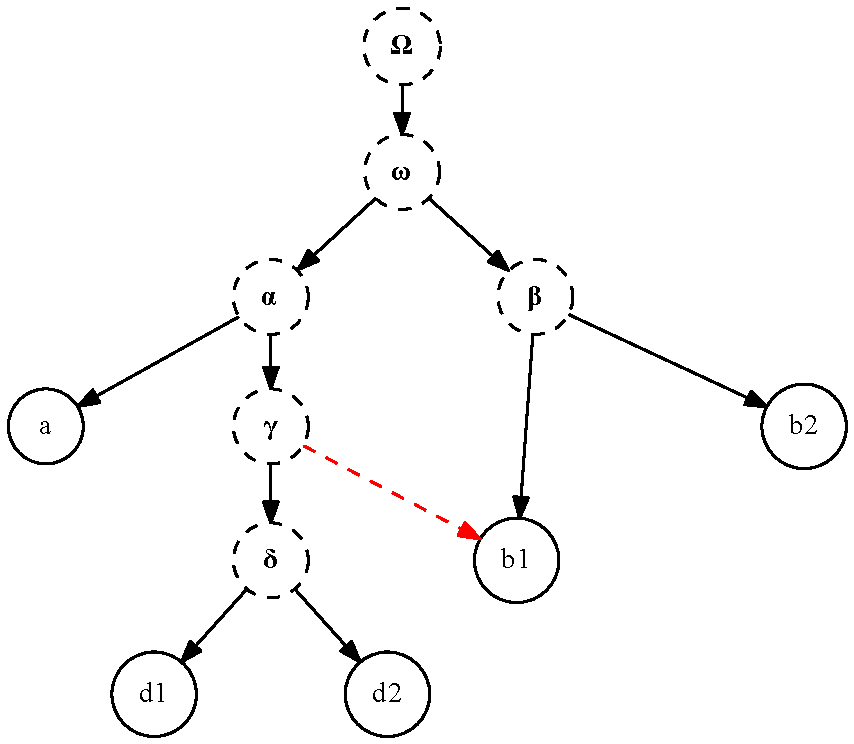
\includegraphics[scale=0.5]{../img/stemma-contamination.pdf}
		\end{center}
	\end{frame}
	\begin{frame}
		\onslide<2->{\hfill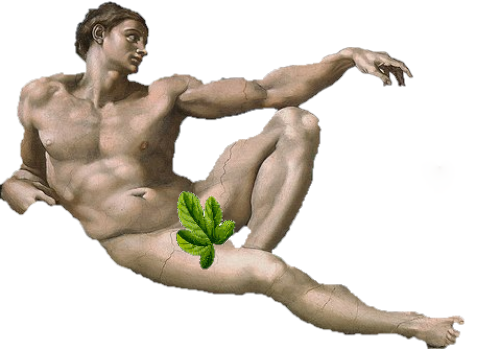
\includegraphics[scale=0.2]{../img/adam.png}}
		\begin{itemize}
			\item Key assumption: \emph{no hypothetical ancestors} (except the \emph{Ausgangstext} A)
			\item Other important assumptions:
			\begin{enumerate}
				\item Scribes typically copied their exemplars with fidelity.
				\item If a scribe introduced a variant, then it came from some other reading.
				\item Scribes typically used fewer sources rather than many.
				\item Scribes typically used closely related sources rather than distant ones.
			\end{enumerate}
		\end{itemize}
	\end{frame}
	\begin{frame}
		\begin{itemize}
			\item \emph{Not} a new methodology for evaluating variant readings, but a ``meta-approach'' to be used on top of existing methods			
			\item \emph{Not} a way to make computers do textual criticism, but a way for them to help us refine human judgments
		\end{itemize}
	\end{frame}
	\section*{Roadmap}
	\begin{frame}
		\begin{itemize}
			\item ``Iterative workflow'' highlighted in blue
		\end{itemize}
		\begin{center}
			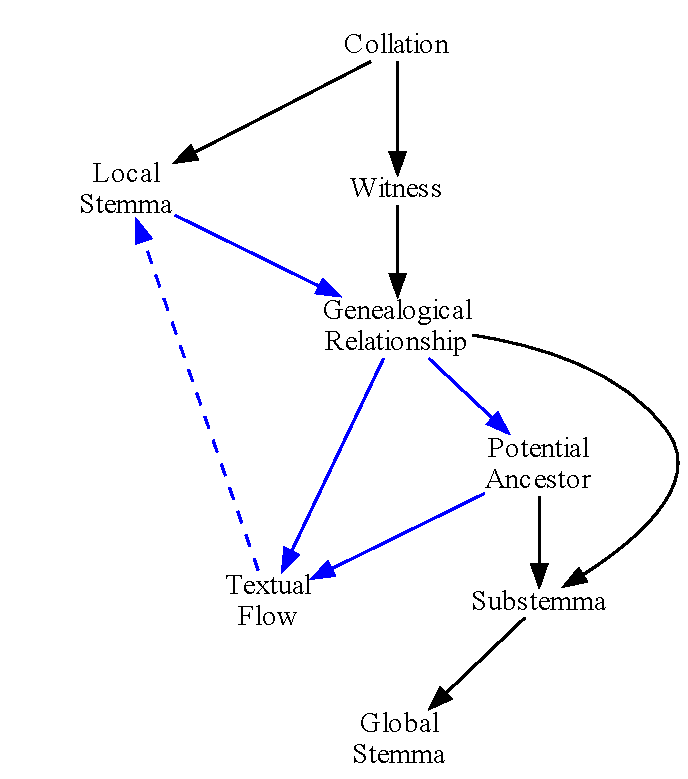
\includegraphics[width=0.5\textwidth]{../img/roadmap.pdf}
		\end{center}
	\end{frame}
	\section*{Collation}
	\begin{frame}
		\begin{itemize}
			\item To compare manuscripts' texts, we must first align them at independent \emph{variation units}
			\item \emph{Variant readings} occur at variation units
		\end{itemize}
		\begin{center}
			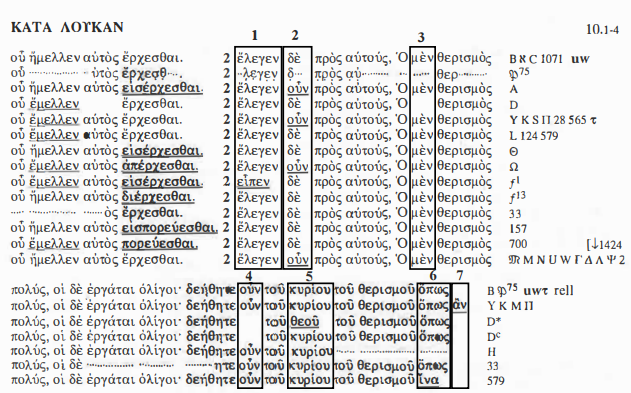
\includegraphics[width=0.75\textwidth]{../img/swanson-luke-10-2-variation-units.png}
		\end{center}
		\footnotesize\parencite[Source:][183]{Swanson.Luke}
	\end{frame}
	\begin{frame}
		\begin{itemize}
			\item Variation units serve as our points of comparison between witnesses in the CBGM
			\item Think of them as the columns of a table and the witnesses as rows
		\end{itemize}
		\begin{center}
			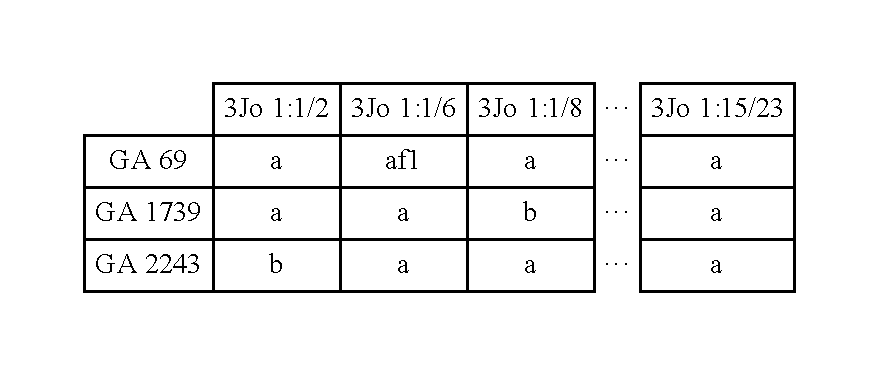
\includegraphics[scale=0.5]{../img/witnesses.pdf}
		\end{center}
	\end{frame}
	\begin{frame}
		\begin{itemize}
			\item This is readily encoded in TEI XML format
		\end{itemize}
		\begin{center}
			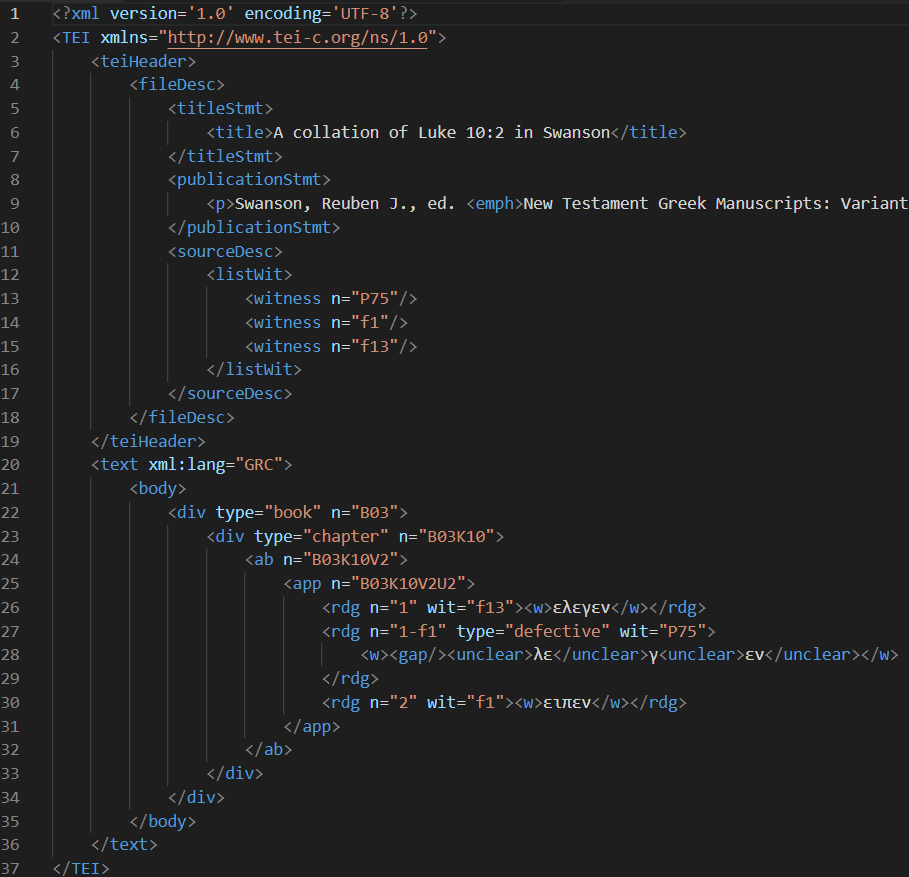
\includegraphics[width=0.65\textwidth]{../img/collation-xml.png}
		\end{center}
	\end{frame}
	\begin{frame}[fragile]
		\begin{columns}
			\begin{column}{0.25\textwidth}
				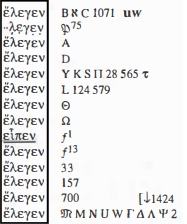
\includegraphics[width=\textwidth]{../img/swanson-luke-10-2-2.png}
			\end{column}
			\begin{column}{0.65\textwidth}
				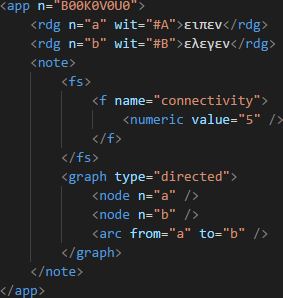
\includegraphics[width=\textwidth]{../img/app-xml.png}
			\end{column}
		\end{columns}
		\begin{center}
\begin{verbatim}
                        reading_support = {
                            "f13": "1",
                            "P75": "1-f1",
                            "f1": "2"
                        }
\end{verbatim}
		\end{center}
	\end{frame}
	\section*{The Local Stemma}
	\begin{frame}
		\begin{itemize}
			\item The basic unit of comparison
			\item One for each variation unit
			\item A graphical representation of our judgments of readings
			\item Kurt Aland's ``local genealogical'' principle
		\end{itemize}
		\begin{columns}
			\begin{column}{0.45\textwidth}
				\begin{center}
					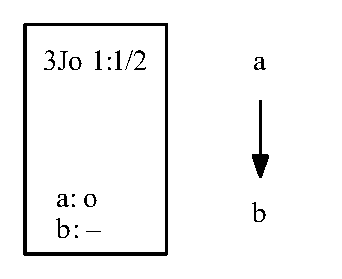
\includegraphics[scale=0.5]{../img/B25K1V1U2-local-stemma.pdf}
				\end{center}
			\end{column}
			\begin{column}{0.45\textwidth}
				\begin{center}
					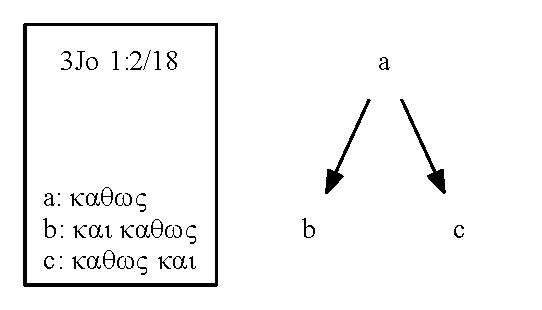
\includegraphics[scale=0.5]{../img/B25K1V2U18-local-stemma.pdf}
				\end{center}
			\end{column}
		\end{columns}
	\end{frame}
	\begin{frame}
		\begin{itemize}
			\item Some are more complicated
			\begin{itemize}
				\item \emph{defective} readings (e.g., misspellings, reconstructions)
				\item \emph{orthographic} readings (e.g., regional differences)
				\item \emph{split} attestations of the same reading (coincidental emergence)
				\item \emph{ambiguous} readings (can be reconstructed as more than one reading)
			\end{itemize}
			\item Some of these may be collapsed with other substantive readings
			\begin{center}
				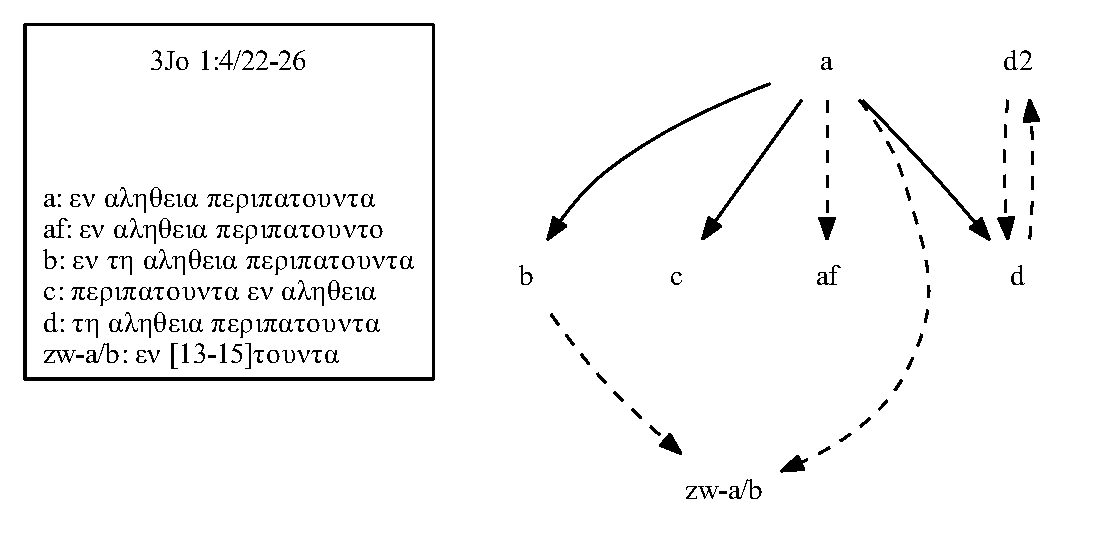
\includegraphics[scale=0.5]{../img/B25K1V4U22-26-local-stemma-ignore-defective-ignore-ambiguous-merge-splits.pdf}
			\end{center}
		\end{itemize}
	\end{frame}
	\begin{frame}
		\begin{columns}
			\begin{column}{0.55\textwidth}
				\begin{itemize}
					\item Computationally, just a directed graph.
				\end{itemize}
				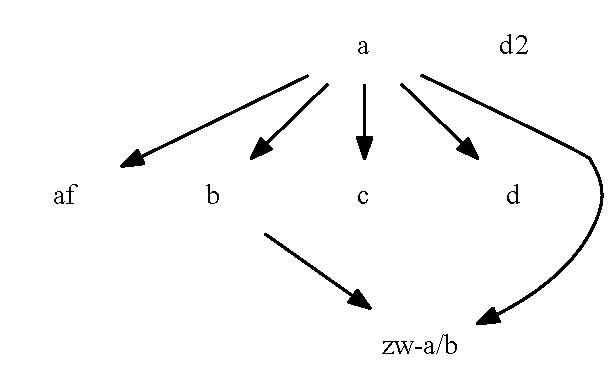
\includegraphics[width=\textwidth]{../img/B25K1V4U22-26-local-stemma-no-legend.pdf}
			\end{column}
			\begin{column}{0.4\textwidth}
				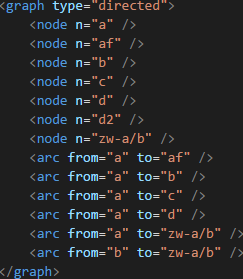
\includegraphics[scale=0.6667]{../img/local-stemma-xml.png}
			\end{column}
		\end{columns}
	\end{frame}
	\begin{frame}
		\begin{itemize}
			\item Relationships between readings are determined by checking for a path between them
			\item $a = b$ (agreement): path of length $0$
			\item $a > b$ (prior): path of length $> 0$ from $a$ to $b$
			\item $a < b$ (posterior): path of length $> 0$ from $b$ to $a$
			\item NOREL (no relationship): no path from $a$ to $b$, but both have a \emph{common ancestor}
		\end{itemize}
		\begin{center}
			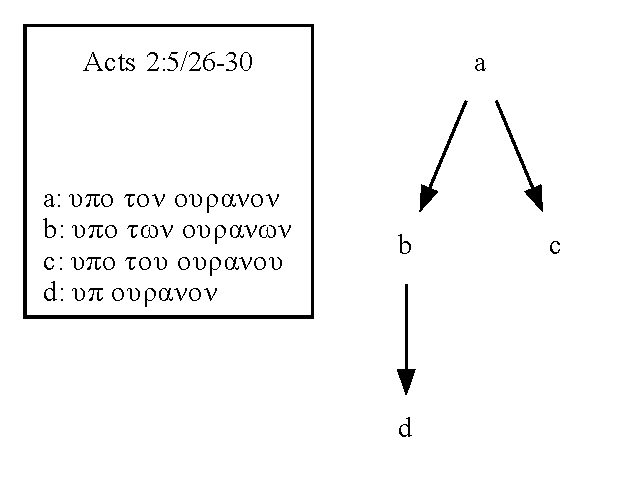
\includegraphics[scale=0.5]{../img/B05K2V5U26-30-local-stemma.pdf}
		\end{center}
	\end{frame}
	\begin{frame}
		\begin{itemize}
			\item UNCL (unclear): same as NOREL, but no common ancestor (reserved for when we don't know where a reading fits in the stemma)
			\item We say that one reading \emph{explains} another if
			\begin{itemize}
				\item it is the same reading (explanation by agreement), or
				\item there is a path of length $1$ from it to the other reading
			\end{itemize}
			\item Lacunae do not have to be explained, and they cannot explain readings
		\end{itemize}
		\begin{center}
			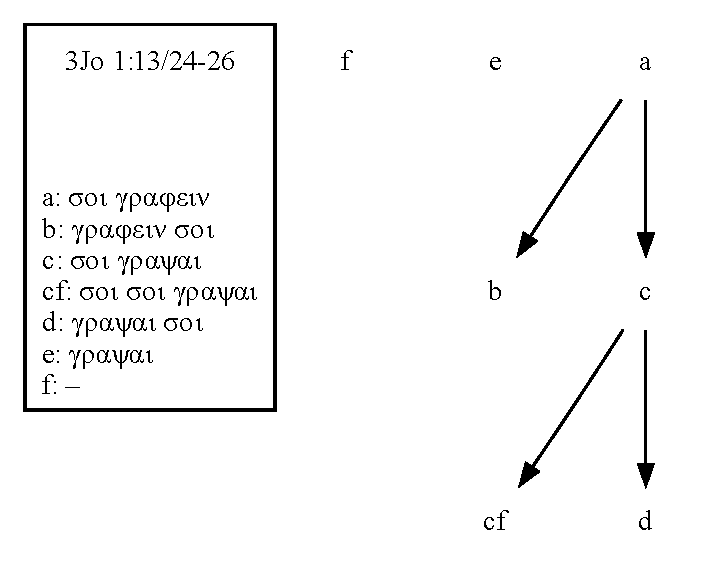
\includegraphics[scale=0.5]{../img/B25K1V13U24-26-local-stemma-incomplete.pdf}
		\end{center}
	\end{frame}
	\section*{Witnesses}
	\begin{frame}
		\begin{itemize}
			\item For the CBGM's purposes, a \emph{witness} is a sequence of readings
			\item Typically, the \emph{text} of a known manuscript, minus the material baggage (date, provenance, etc.)
			\begin{itemize}
				\item ``How texts relate'' $\neq$ ``How manuscripts relate''
			\end{itemize}
		\end{itemize}
		\begin{center}
			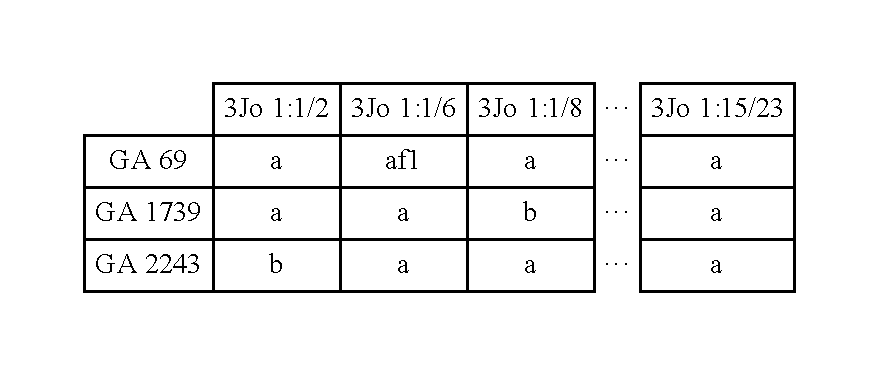
\includegraphics[scale=0.5]{../img/witnesses.pdf}
		\end{center}
	\end{frame}
	\begin{frame}
		\begin{itemize}
			\item Versions and fathers can also be treated as witnesses
			\item But back-translation may be ambiguous, and patristic citations may be ``lacunose''
		\end{itemize}
		\begin{center}
			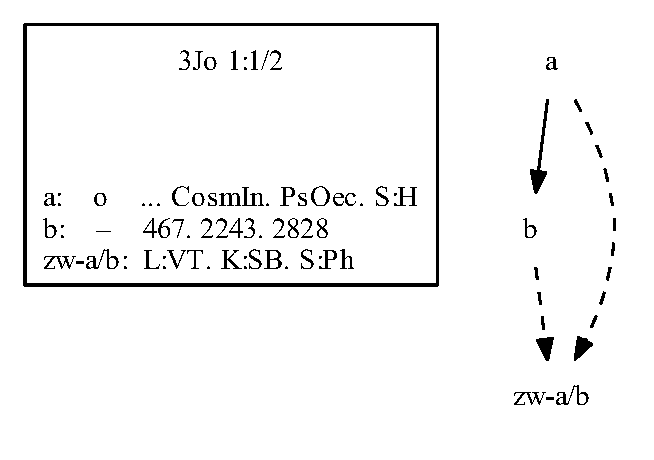
\includegraphics[scale=0.5]{../img/B25K1V1U2-local-stemma-versions-fathers.pdf}
		\end{center}
	\end{frame}
	\section*{Genealogical Relationships}
	\begin{frame}
		\begin{itemize}
			\item The relationship of two witnesses is the overall pattern \emph{of the relationships of their readings} where both are extant
			\item The \emph{cost} of a genealogical relationship is the number of explained readings that are not agreements (so the cost in the example below is $1$)
		\end{itemize}
		\begin{center}
			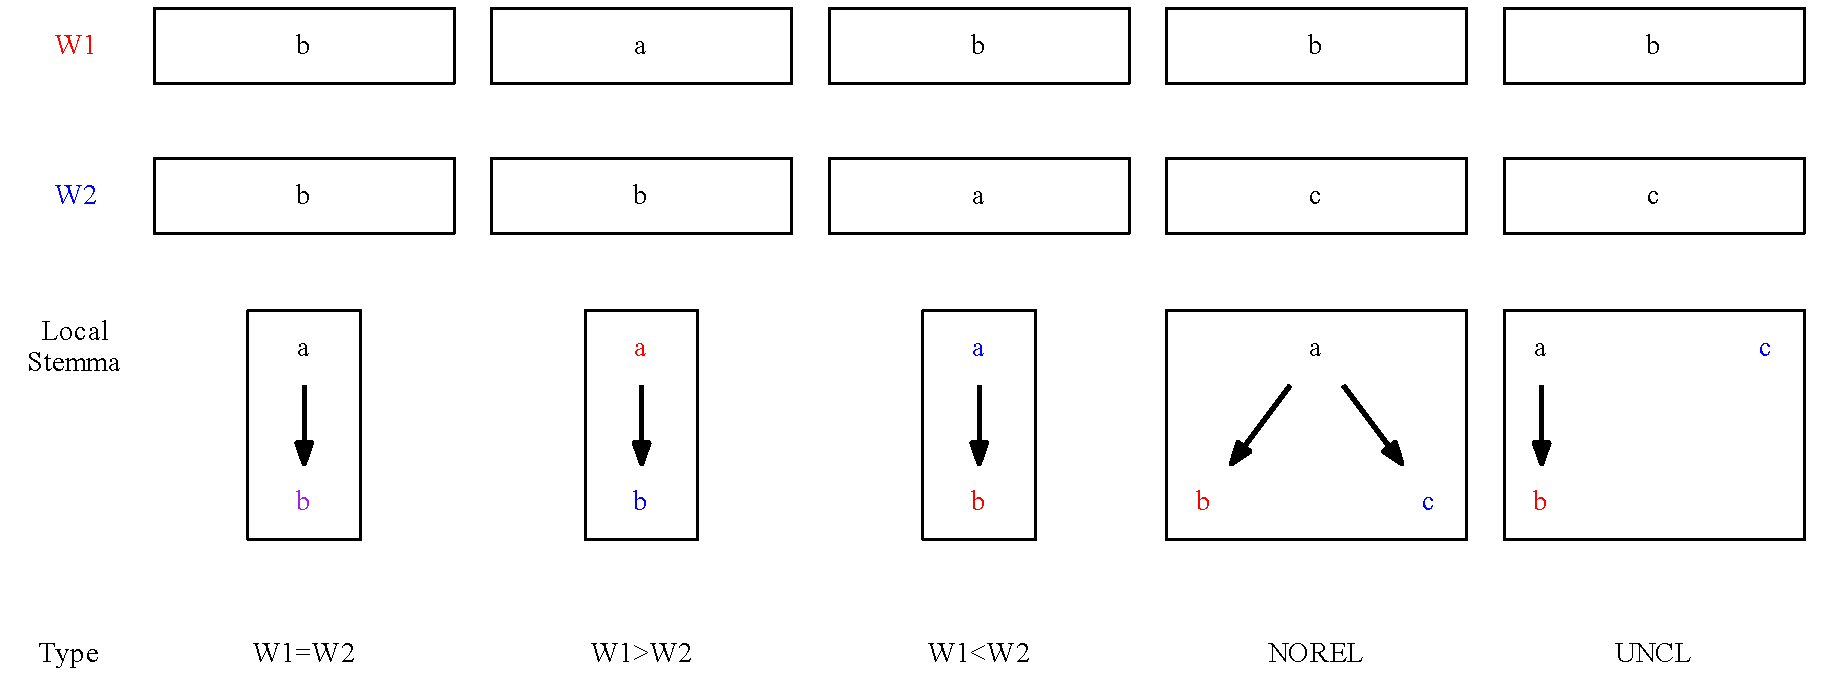
\includegraphics[width=\textwidth]{../img/genealogical-relationships.pdf}
		\end{center}
	\end{frame}
	\begin{frame}
		\begin{itemize}
			\item It is convenient to encode genealogical relationships with \emph{bitmaps}
		\end{itemize}
		\begin{columns}
			\begin{column}{0.45\textwidth}
				\begin{align*}
					\mathtt{agree} &= [1,0,0,0,0]\\
					\mathtt{prior} &= [0,1,0,0,0]\\
					\mathtt{posterior} &= [0,0,1,0,0]\\
					\phantom{*}
				\end{align*}
			\end{column}
			\begin{column}{0.45\textwidth}
				\begin{align*}
					\mathtt{norel} &= [0,0,0,1,0]\\
					\mathtt{uncl} &= [0,0,0,0,1]\\
					\mathtt{expl} &= [1,0,1,0,0]\\
					\mathtt{cost} &= 1
				\end{align*}
			\end{column}
		\end{columns}
		\begin{center}
			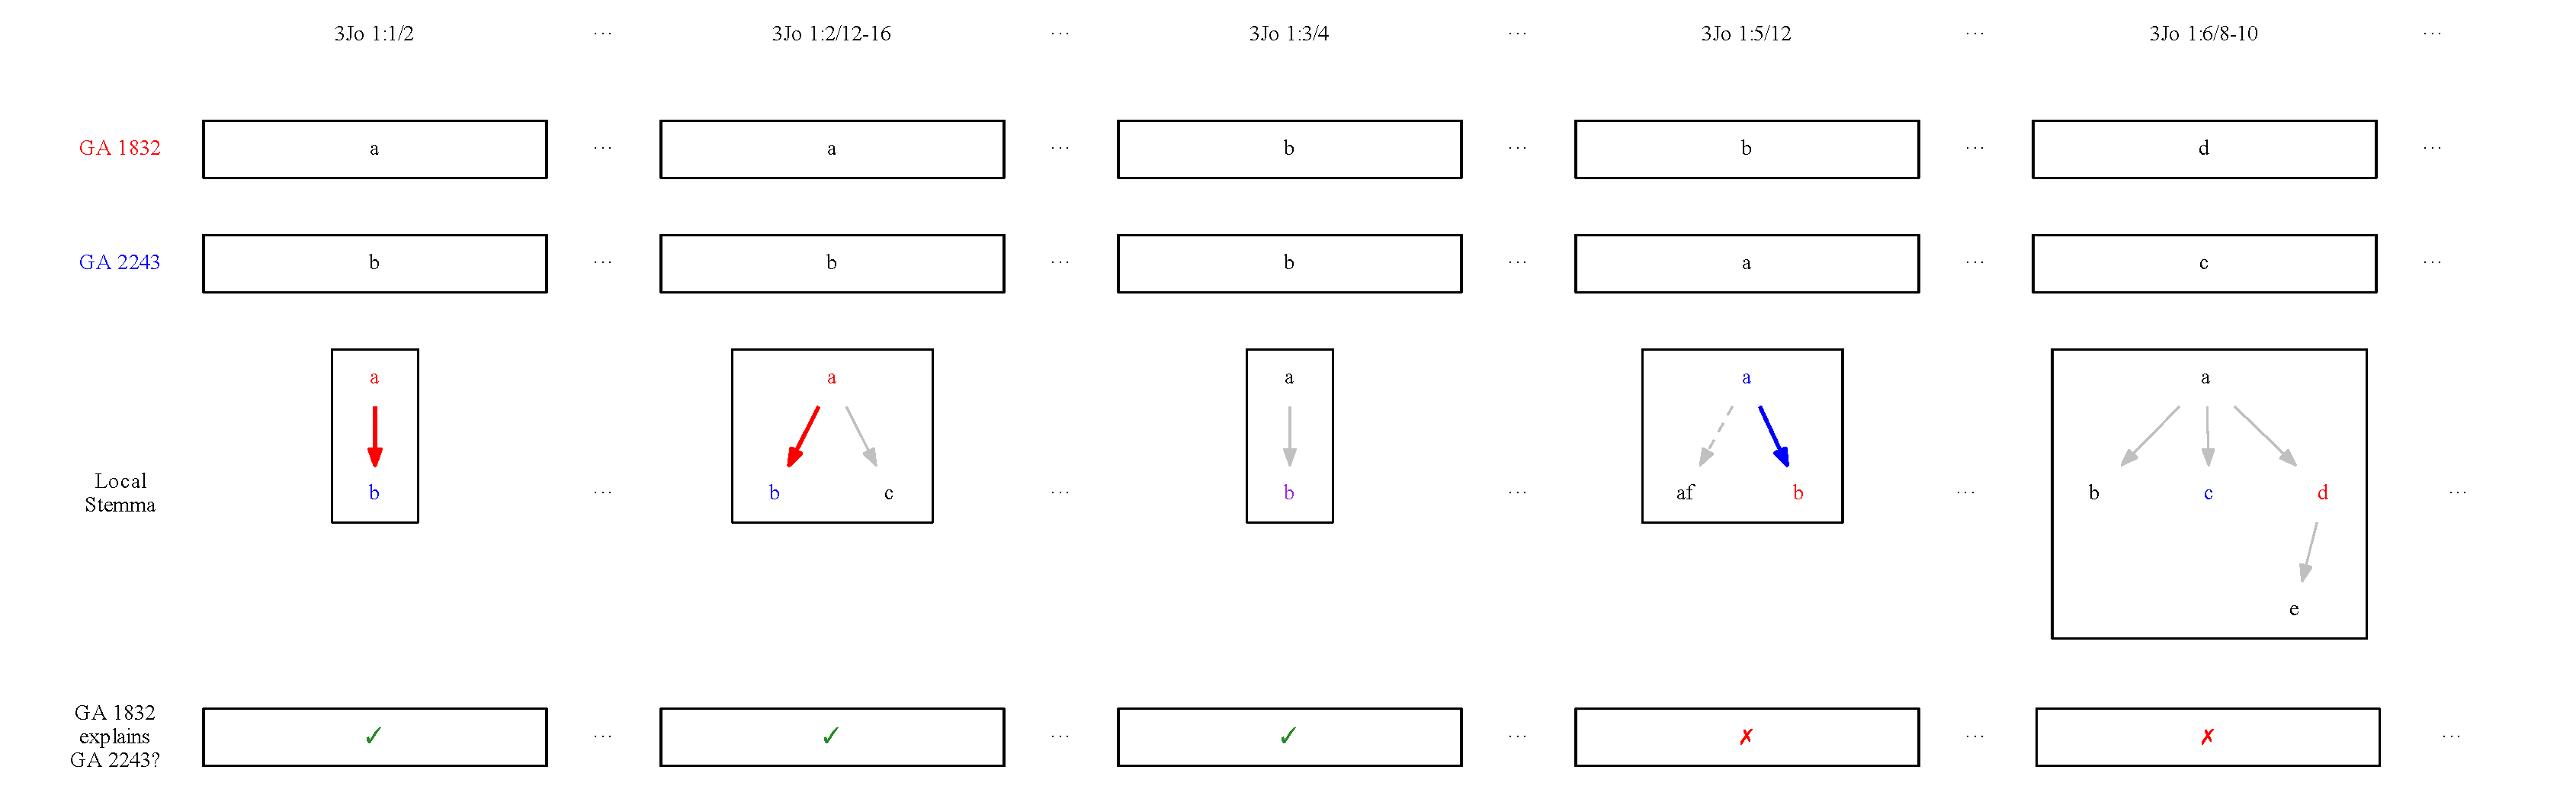
\includegraphics[width=1.125\textwidth]{../img/explained-readings.pdf}
		\end{center}
	\end{frame}
	\begin{frame}
		\begin{itemize}
			\item For $d$ units and $n$ witnesses, $\sim n^2d$ comparisons as one-time work
			\item The \texttt{compare\_witnesses} module (below) presents this computed data
		\end{itemize}
		\begin{center}
			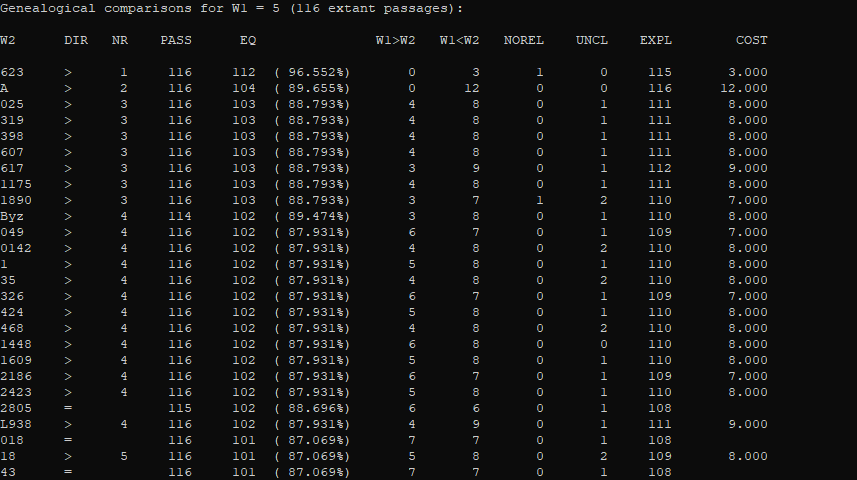
\includegraphics[scale=0.5]{../img/compare-witnesses.png}
		\end{center}
	\end{frame}
	\section*{Potential Ancestors}
	\begin{frame}
		\begin{itemize}
			\item Potential ancestor = ``more prior than posterior readings''
		\end{itemize}
		\begin{center}
			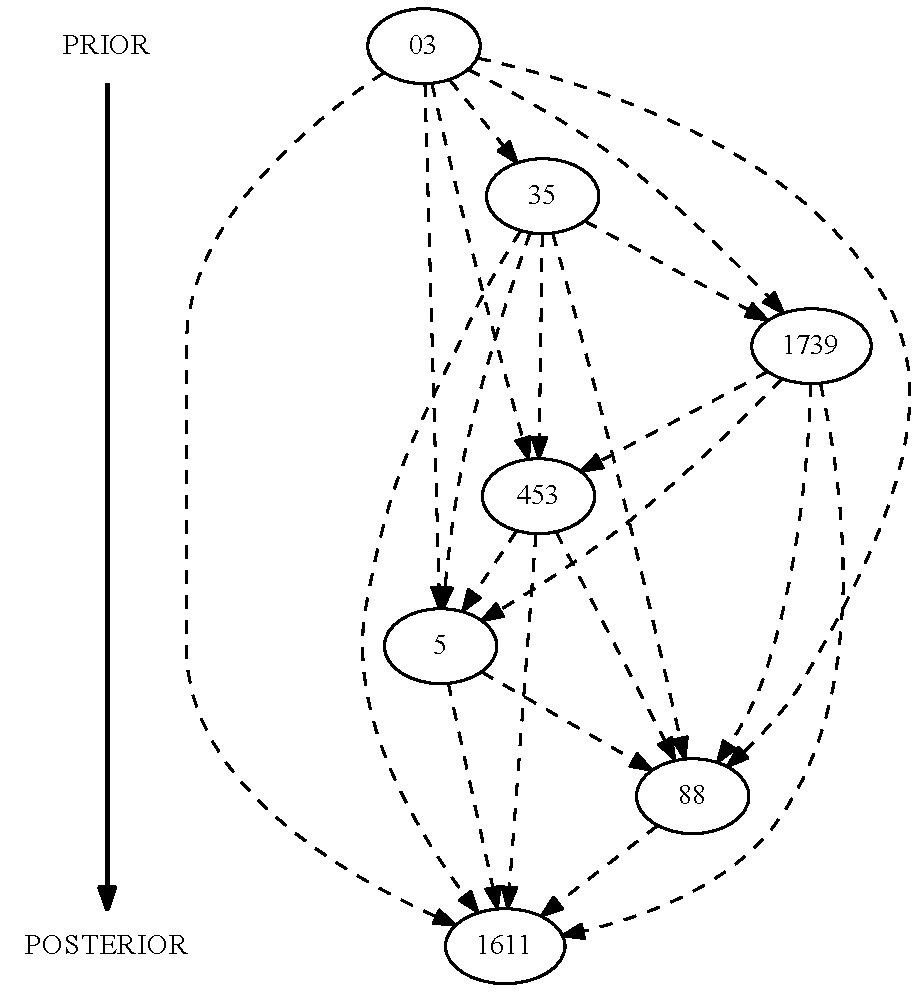
\includegraphics[scale=0.4]{../img/potential-ancestors.pdf}
		\end{center}
	\end{frame}
	\section*{Textual Flow at a Variation Unit}
	\begin{frame}
		\begin{columns}
			\begin{column}{0.45\textwidth}
				\begin{itemize}
					\item \emph{Textual flow} is a tool for helping us revise our judgments in a local stemma
					\item \emph{Not} a global stemma (our ultimate goal), but still important
				\end{itemize}
			\end{column}
			\begin{column}{0.45\textwidth}
				\begin{center}
					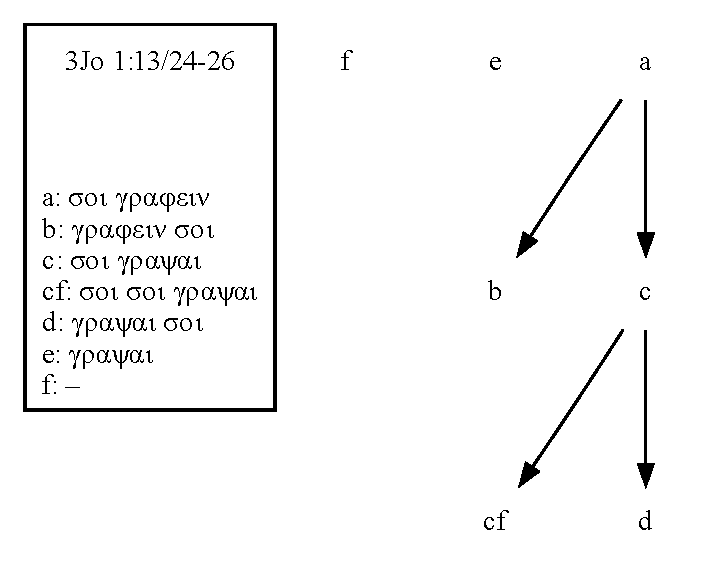
\includegraphics[width=\textwidth]{../img/B25K1V13U24-26-local-stemma-incomplete.pdf}
				\end{center}
			\end{column}
		\end{columns}
		\begin{center}
			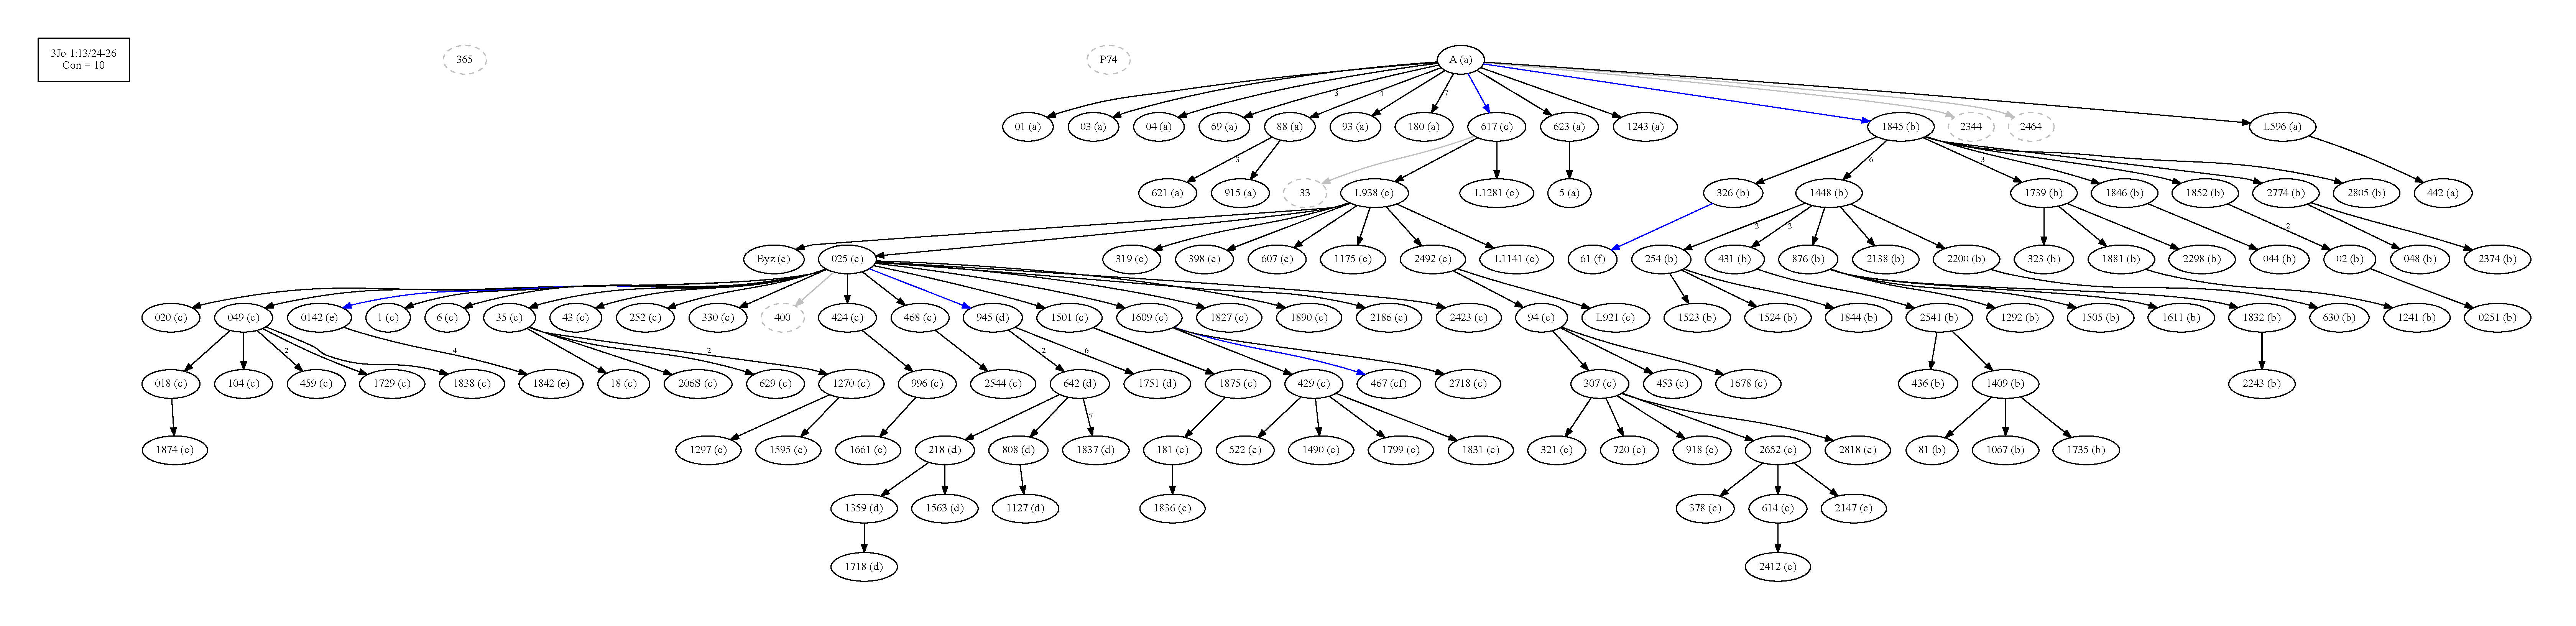
\includegraphics[width=\textwidth]{../img/B25K1V13U24-26-textual-flow.pdf}
		\end{center}
	\end{frame}
	\begin{frame}
		\begin{itemize}
			\item How do we find a given witness's \emph{textual flow ancestor}?
			\item We specify a \emph{connectivity limit} \textgreek{κ} (i.e., a radius of ``close-enough'' neighbors)
			\item Then, for each witness:
			\begin{enumerate}
				\item List its potential ancestors, sorted from most agreement to least
				\item If one of the first \textgreek{κ} has the same reading at this unit, then select it
				\item If not, then choose the first (non-lacunose) potential ancestor
			\end{enumerate}
			\item Core idea: use \emph{general relationships} (between witnesses) to find \emph{specific relationships} (between readings in a local stemma)
		\end{itemize}
	\end{frame}
	\section*{Textual Flow for a Variant Reading}
	\begin{frame}
		\begin{itemize}
			\item Often, we just want to know the textual flow for witnesses with a specific reading
		\end{itemize}
		\begin{center}
			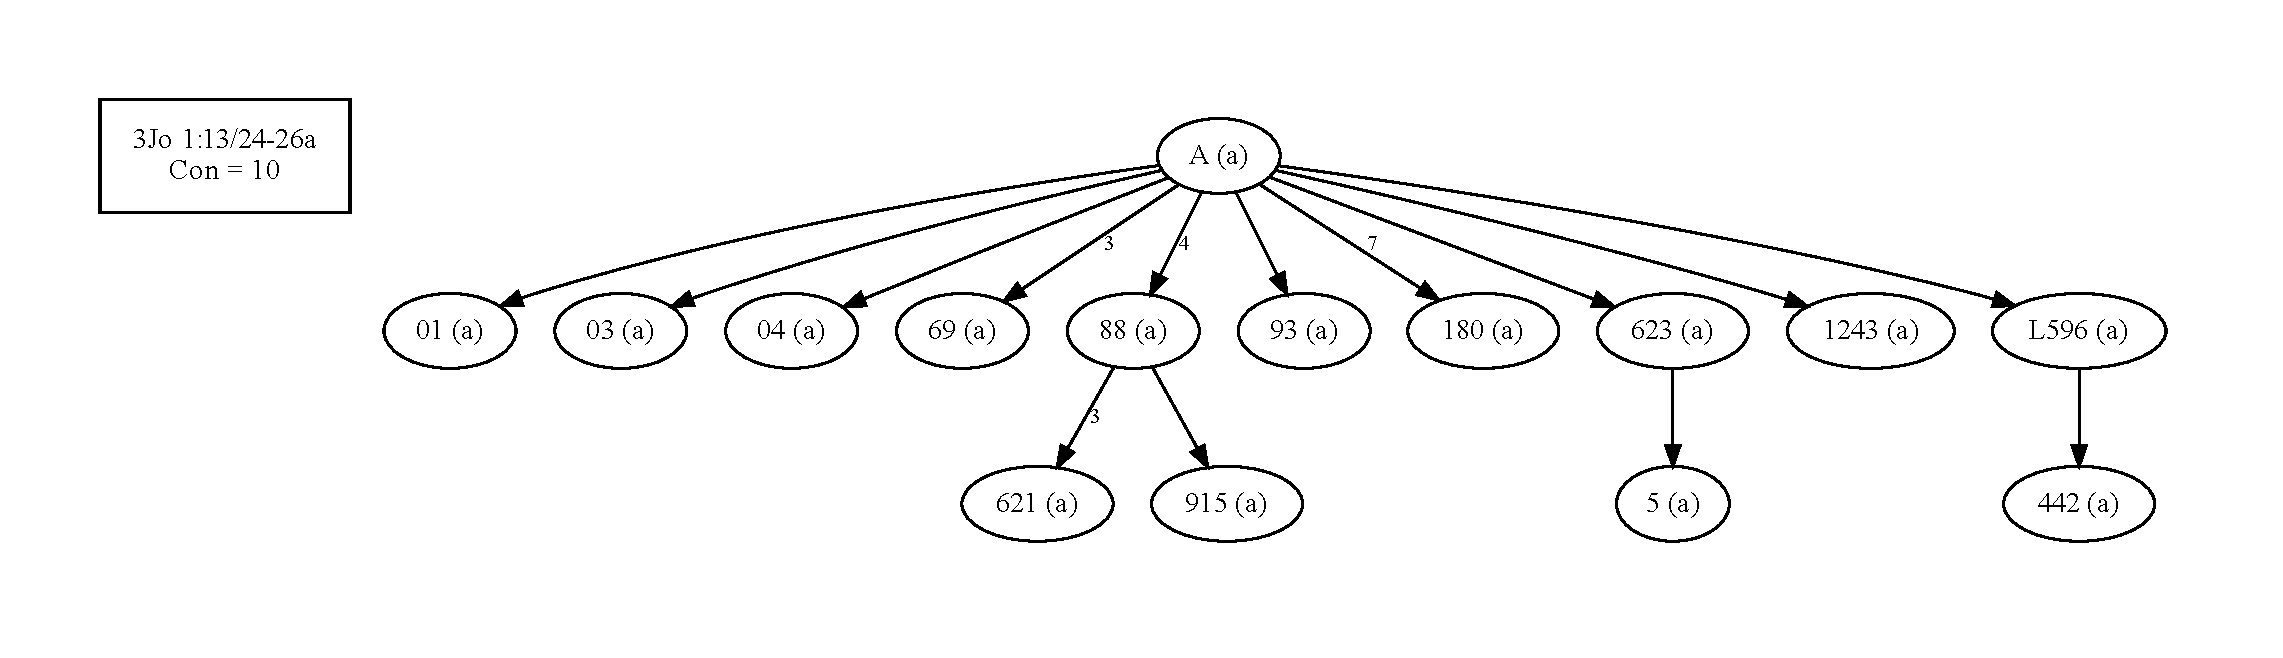
\includegraphics[width=\textwidth]{../img/B25K1V13U24-26Ra-coherence-attestations.pdf}
		\end{center}
		\begin{itemize}
			\item (Numbers on edges represent the rank of the closest potential ancestor with the same reading, if it's not 1)
		\end{itemize}
	\end{frame}
	\begin{frame}
		\begin{itemize}
			\item We can use it to evaluate alternate hypotheses about the initial text (A)
		\end{itemize}
		\begin{columns}
			\begin{column}{0.45\textwidth}
				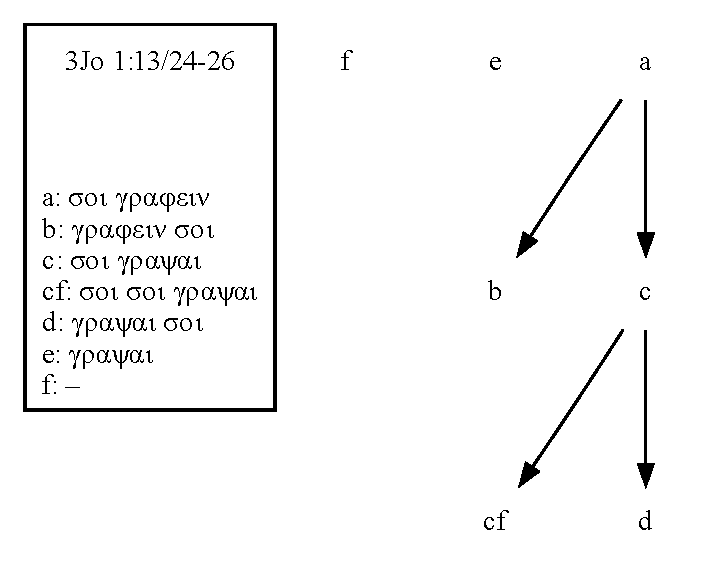
\includegraphics[width=\textwidth]{../img/B25K1V13U24-26-local-stemma-incomplete.pdf}
			\end{column}
			\begin{column}{0.45\textwidth}
				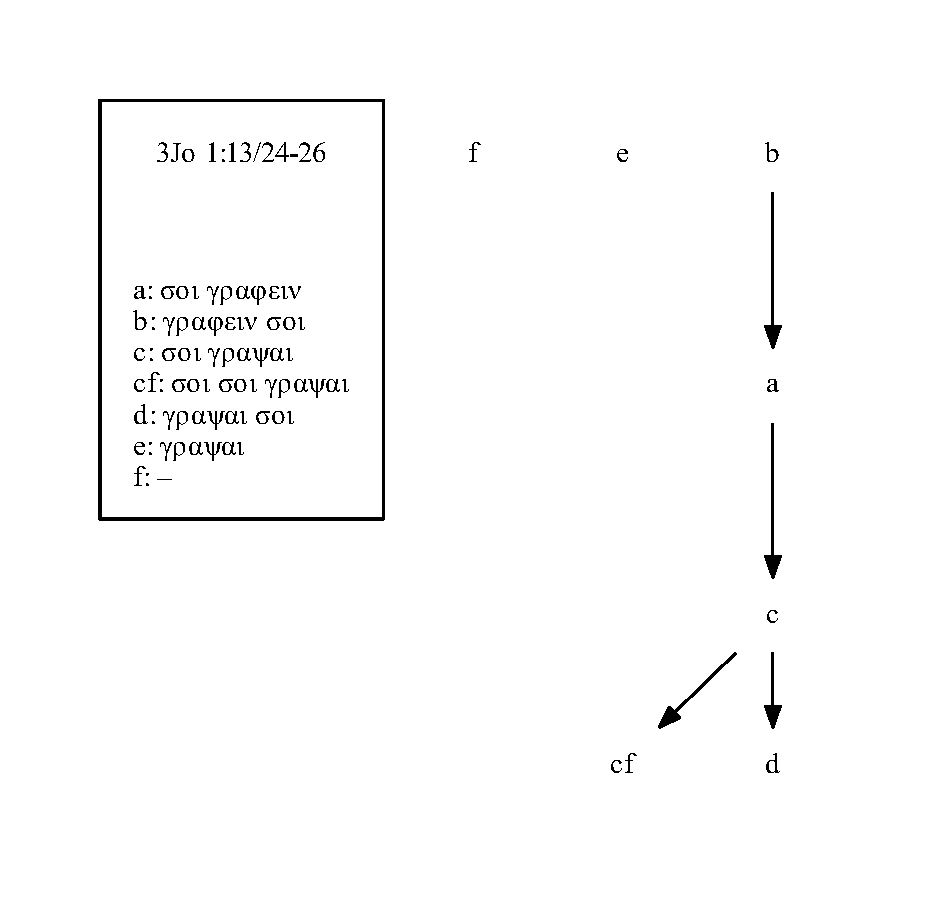
\includegraphics[width=\textwidth]{../img/B25K1V13U24-26-local-stemma-b-initial.pdf}
			\end{column}
		\end{columns}
	\end{frame}
	\begin{frame}
		\begin{center}
			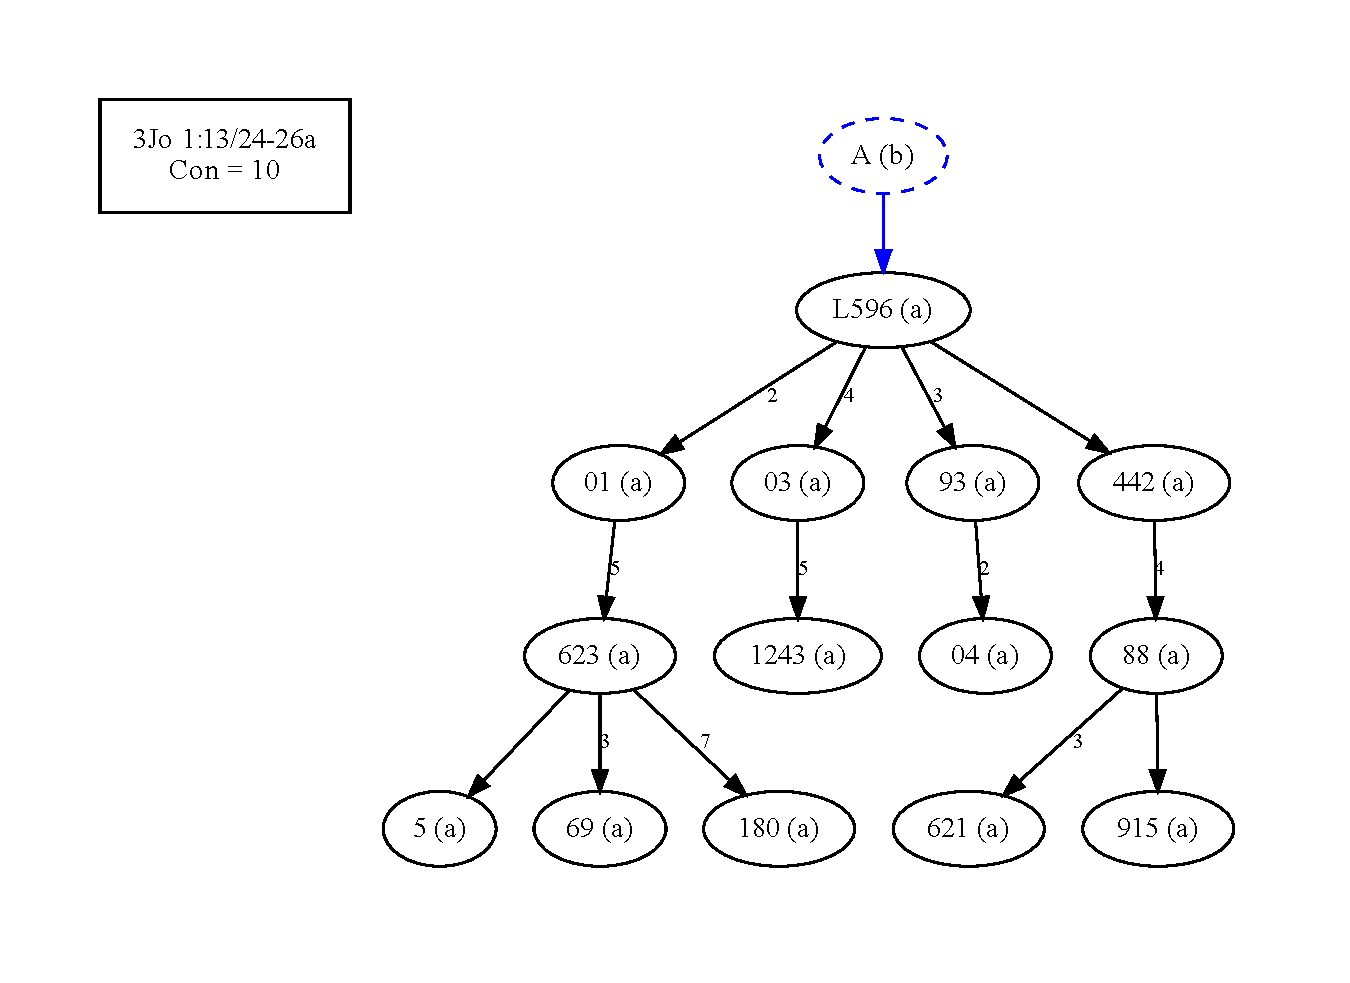
\includegraphics[width=\textwidth]{../img/B25K1V13U24-26Ra-coherence-attestations-b-initial.pdf}
		\end{center}
	\end{frame}
	\begin{frame}
		\begin{columns}
			\begin{column}{0.45\textwidth}
				\begin{itemize}
					\item Or, we can look only at the parts of textual flow where a reading gets changed to find the most likely sources of unexplained readings (\emph{e} and \emph{f})
				\end{itemize}
			\end{column}
			\begin{column}{0.45\textwidth}
				\begin{center}
					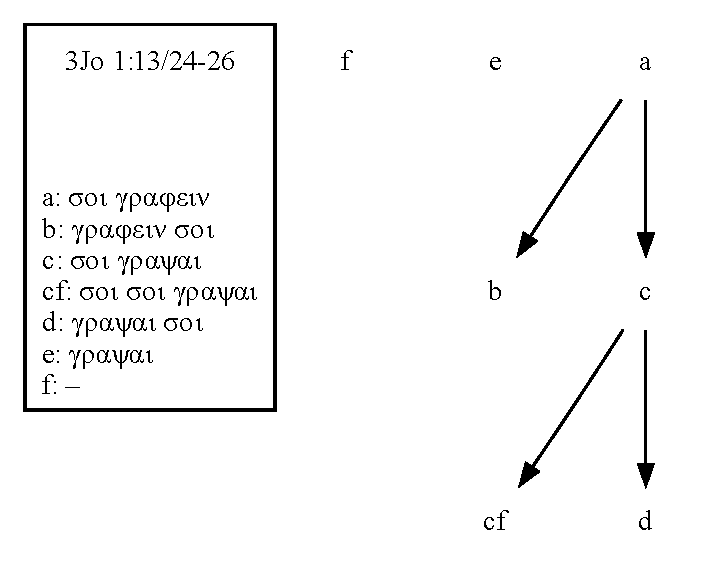
\includegraphics[width=\textwidth]{../img/B25K1V13U24-26-local-stemma-incomplete.pdf}
				\end{center}
			\end{column}
		\end{columns}
	\end{frame}
	\begin{frame}
		\begin{columns}
			\begin{column}{0.45\textwidth}
				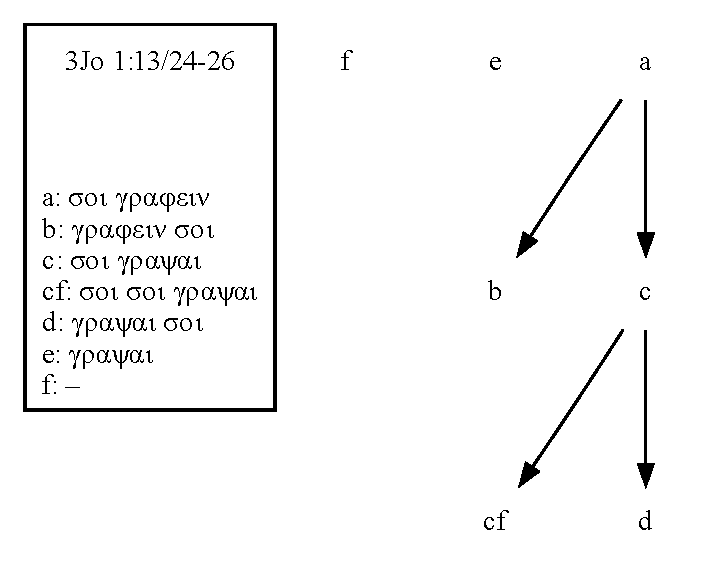
\includegraphics[width=\textwidth]{../img/B25K1V13U24-26-local-stemma-incomplete.pdf}
			\end{column}
			\begin{column}{0.5\textwidth}
				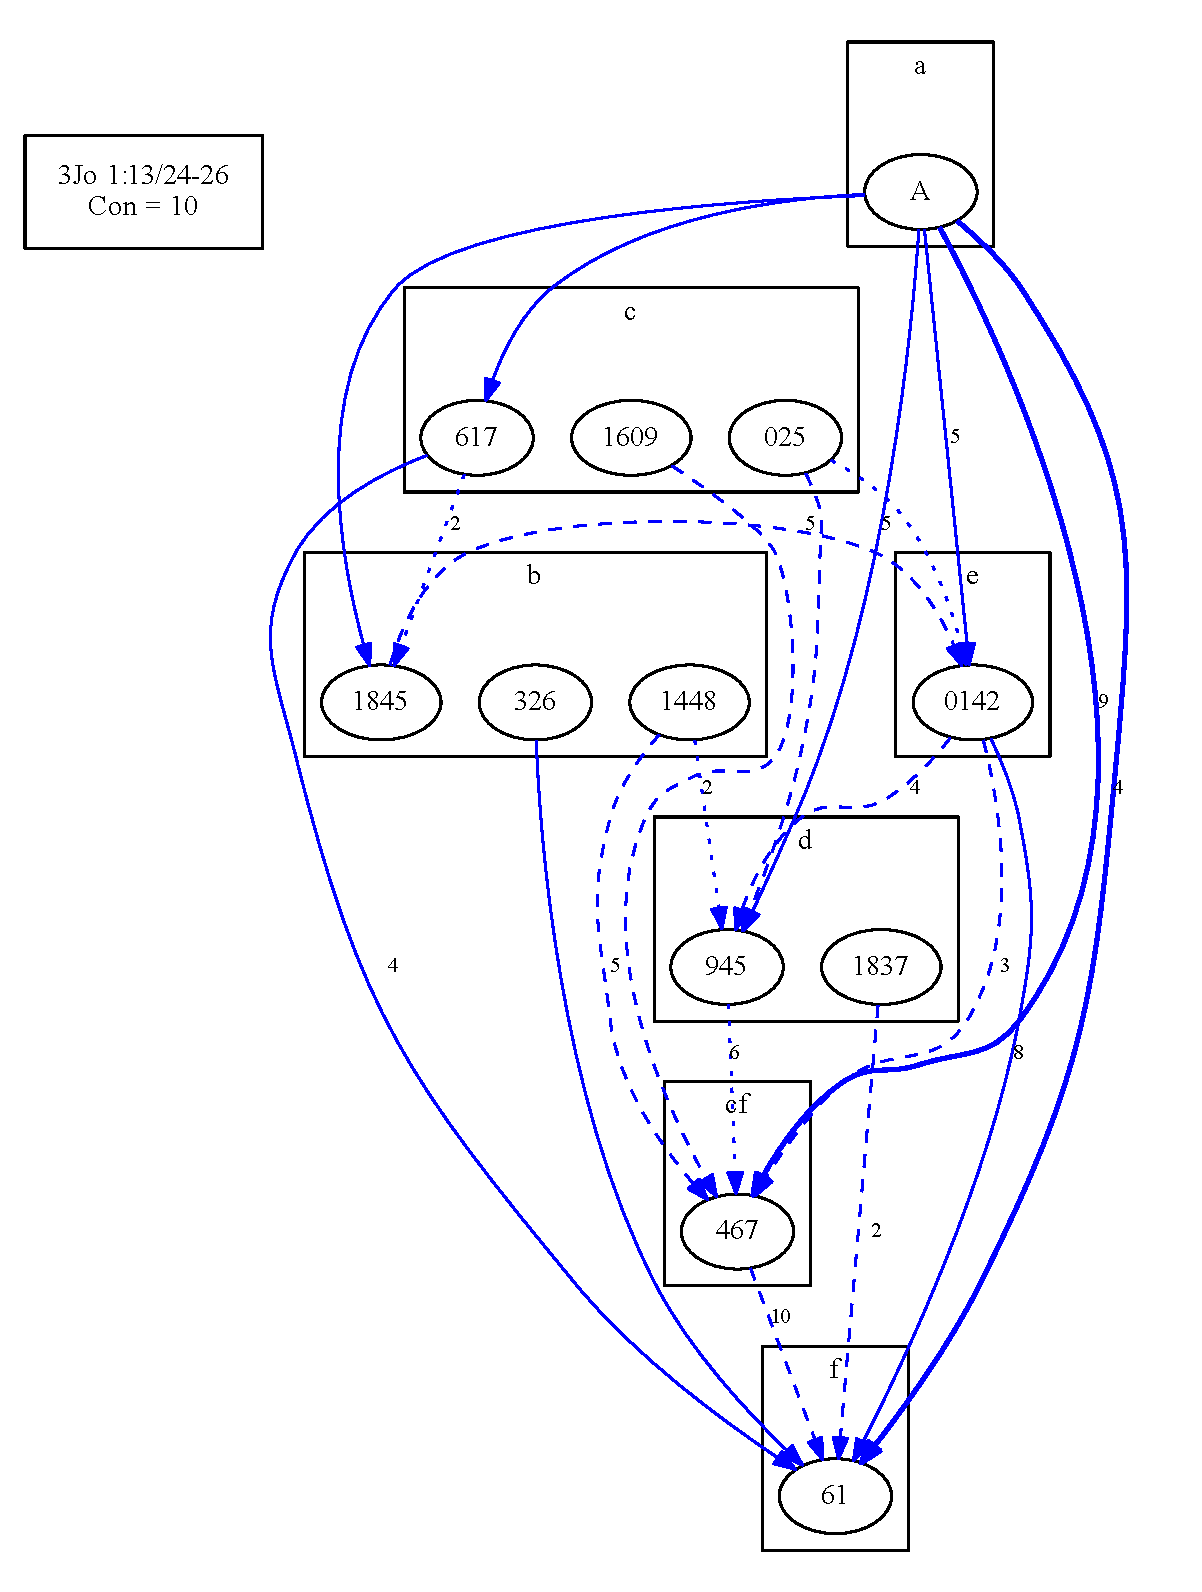
\includegraphics[width=\textwidth]{../img/B25K1V13U24-26-coherence-variants-strengths.pdf}
			\end{column}
		\end{columns}
	\end{frame}
	\begin{frame}
		\begin{columns}
			\begin{column}{0.45\textwidth}
				\begin{itemize}
					\item Between coherence (a form of external evidence) and internal evidence, we can attempt to explain previous unexplained readings
					\item A necessary step for our ultimate goal of constructing a global stemma
				\end{itemize}
			\end{column}
			\begin{column}{0.45\textwidth}
				\begin{center}
					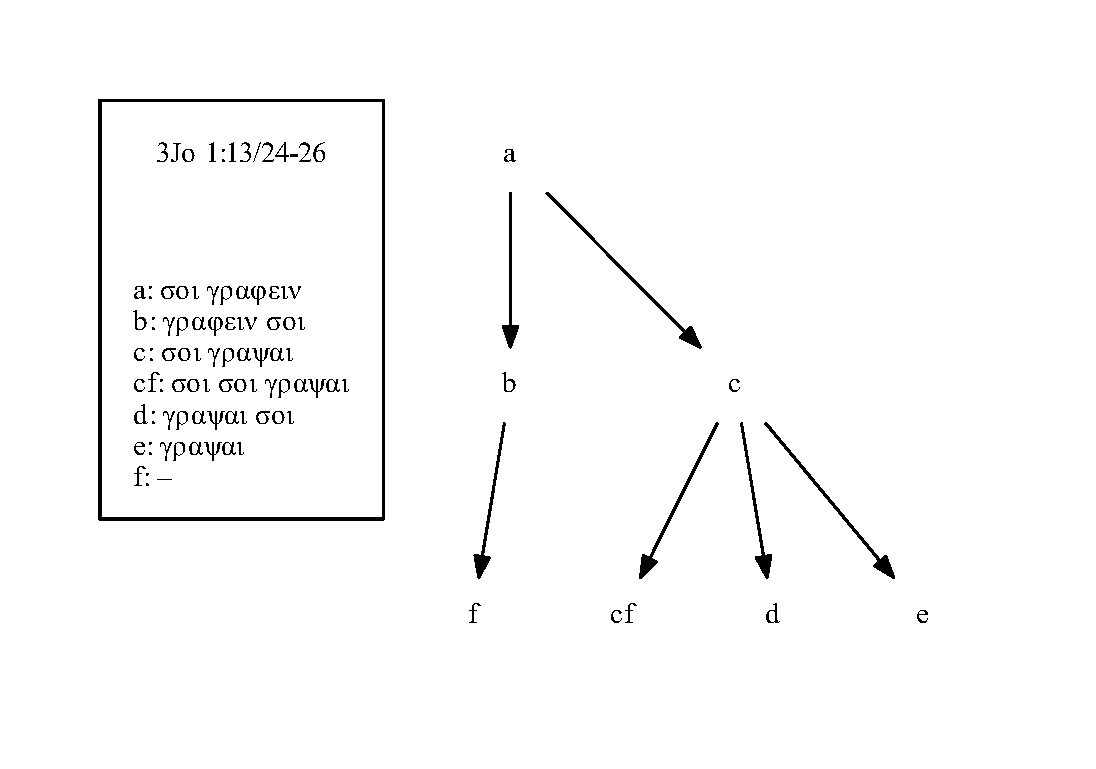
\includegraphics[width=\textwidth]{../img/B25K1V13U24-26-local-stemma-complete.pdf}
				\end{center}
			\end{column}
		\end{columns}
	\end{frame}
%	\section*{Explained Readings}
%	\begin{frame}
%		\begin{columns}
%			\begin{column}{0.4\textwidth}
%				\centering
%				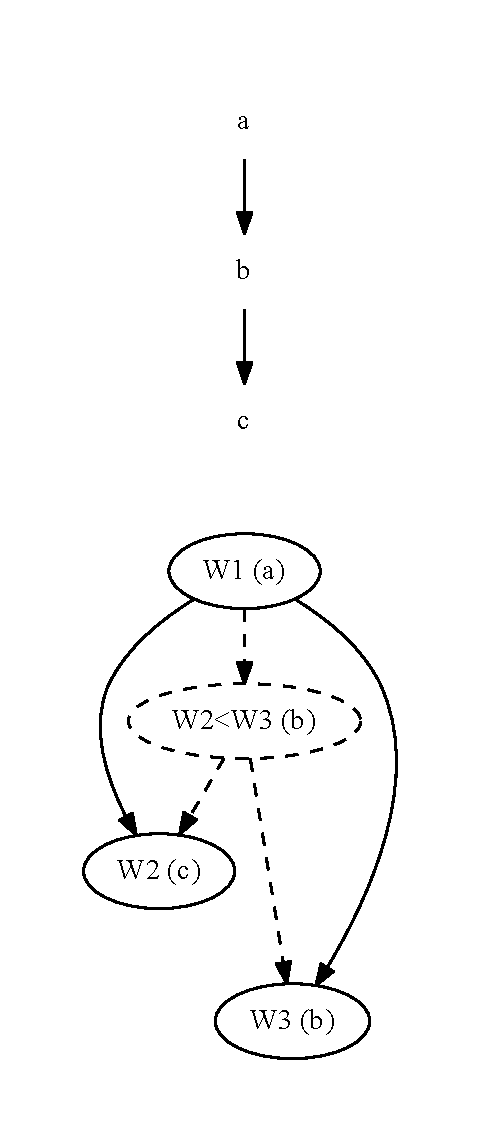
\includegraphics[width=0.75\textwidth]{../img/intermediary-node-example.pdf}
%			\end{column}
%			\begin{column}{0.55\textwidth}
%				\begin{itemize}
%					\item Does a reading explain any of its posterior readings transitively (i.e., in the local stemma to the left, does \emph{a} explain \emph{c})?
%					\item As originally formulated, \emph{no}: \emph{a} explains \emph{b} and \emph{b} explains \emph{c}, but \emph{a} does not explain \emph{c} (it's too many steps removed)
%					\item Later, in the global stemma, \emph{intermediary nodes} may be needed to ensure that all readings are explained
%				\end{itemize}
%			\end{column}
%		\end{columns}
%	\end{frame}
%	\begin{frame}
%		\begin{columns}
%			\begin{column}{0.4\textwidth}
%				\centering
%				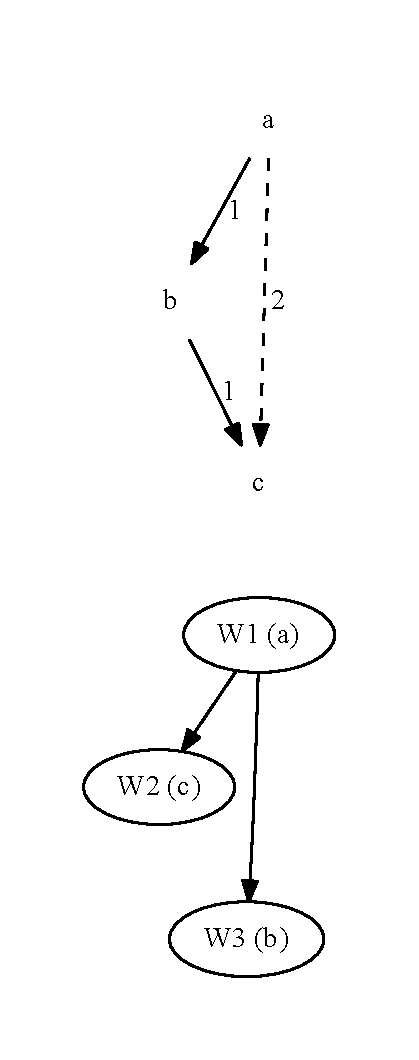
\includegraphics[width=0.75\textwidth]{../img/transitivity-example.pdf}
%			\end{column}
%			\begin{column}{0.55\textwidth}
%				\begin{itemize}
%					\item If we instead allow \emph{a} to explain \emph{c}, but at a higher cost (more on this in the substemma slides), then we remove the need for intermediary nodes (although multiple changes in the same variation unit may be implied along an edge in the global stemma)
%				\end{itemize}
%			\end{column}
%		\end{columns}
%	\end{frame}
	\section*{The Substemma(ta) of a Witness}
	\begin{frame}
		\begin{itemize}
			\item The \emph{substemma} of a witness is the portion of the global stemma consisting of the witness and its ancestors in the stemma
			\item Requirement: \emph{every} extant reading in the witness must be explained by a reading in at least one of its ancestors
		\end{itemize}
		\begin{center}
			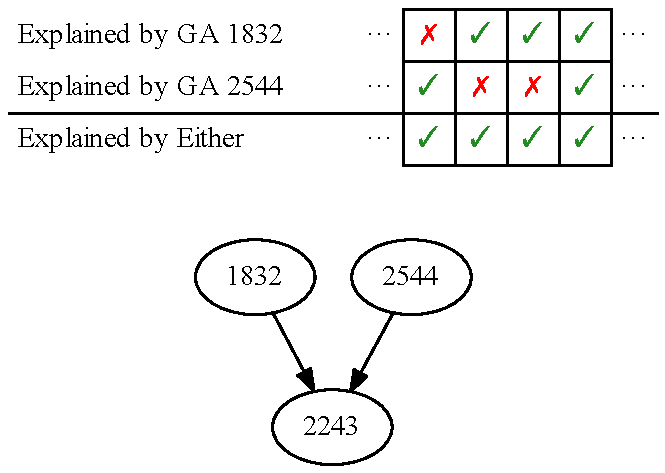
\includegraphics[width=0.6667\textwidth]{../img/ga-2243-substemma.pdf}
		\end{center}
	\end{frame}
	\begin{frame}
		\begin{itemize}
			\item A witness may have multiple valid substemma (i.e., ones that explain all of its readings), but some are better than others
			\item Two of the CBGM's methodological assumptions are important here:
			\begin{enumerate}
				\setcounter{enumi}{2} % manually set the enumerate counter so that the first item is #3
				\item Scribes typically used fewer sources rather than many.
				\item Scribes typically used closely related sources rather than distant ones.
			\end{enumerate}
			\item A balancing act: the substemma \{L938\} is more parsimonious, but may not explain as many readings by agreement
		\end{itemize}
		\begin{center}
			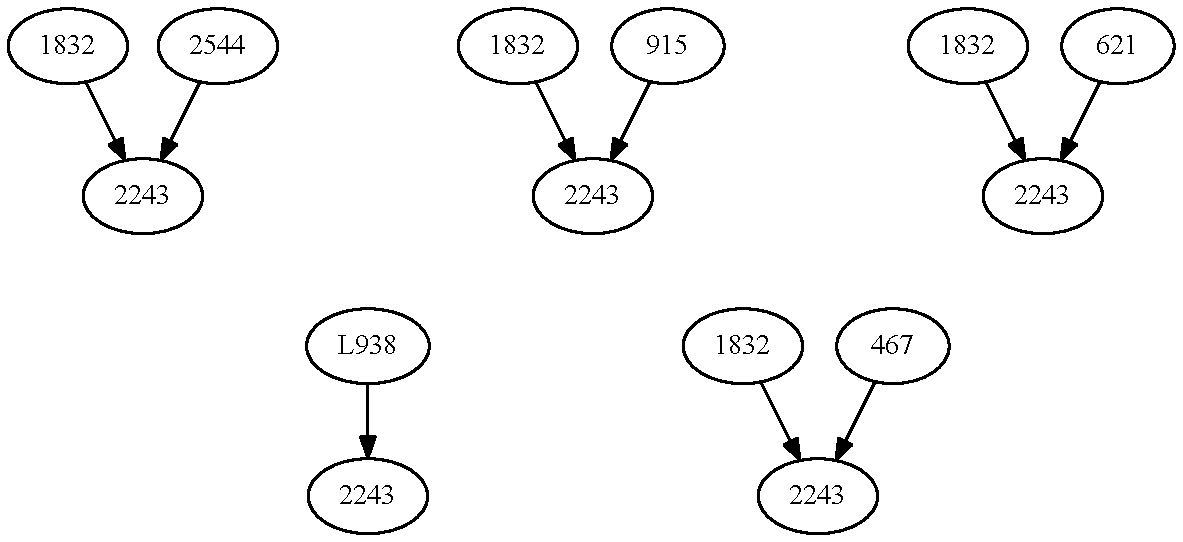
\includegraphics[width=0.75\textwidth]{../img/substemmata.pdf}
		\end{center}
	\end{frame}
%	\begin{frame}
%		\begin{itemize}
%			\item Based on assumption 3, we should prefer substemmata with fewer ancestors (``parsimony'')
%			\item Based on assumption 4, we should prefer substemmata with ancestors that agree as often as possible with the witness
%			\item A balancing act: the substemma \{L938\} is more parsimonious, but may not explain as many readings by agreement
%		\end{itemize}
%		\begin{center}
%			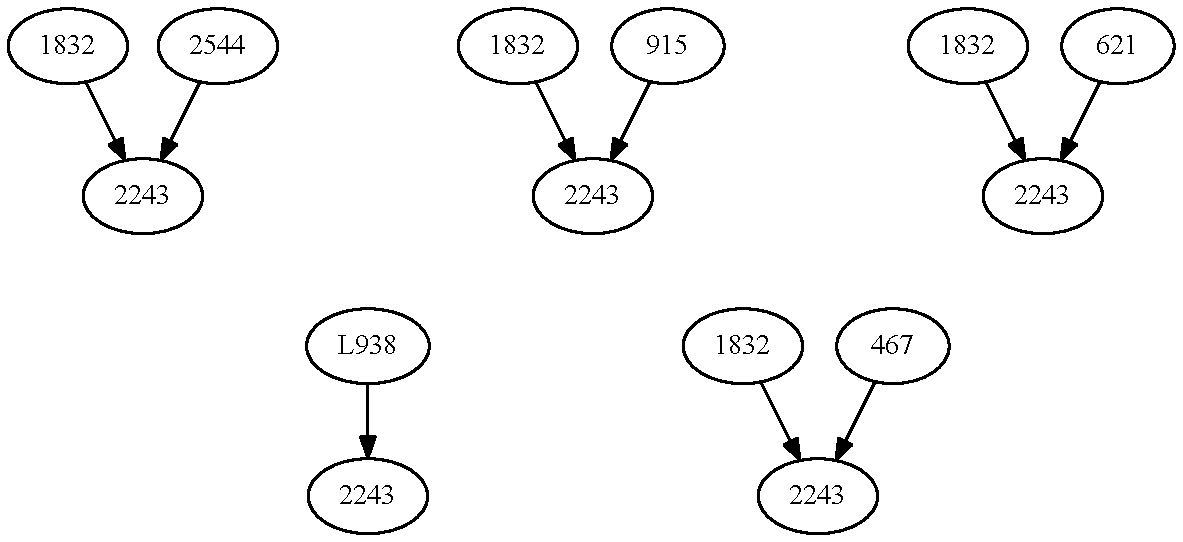
\includegraphics[width=0.75\textwidth]{../img/substemmata.pdf}
%		\end{center}
%	\end{frame}
%	\begin{frame}
%		\begin{itemize}
%			\item A simple cost function for each ancestor is ``the number of variation units where the ancestor explains the witness by descent and not agreement''
%		\end{itemize}
%		\begin{center}
%			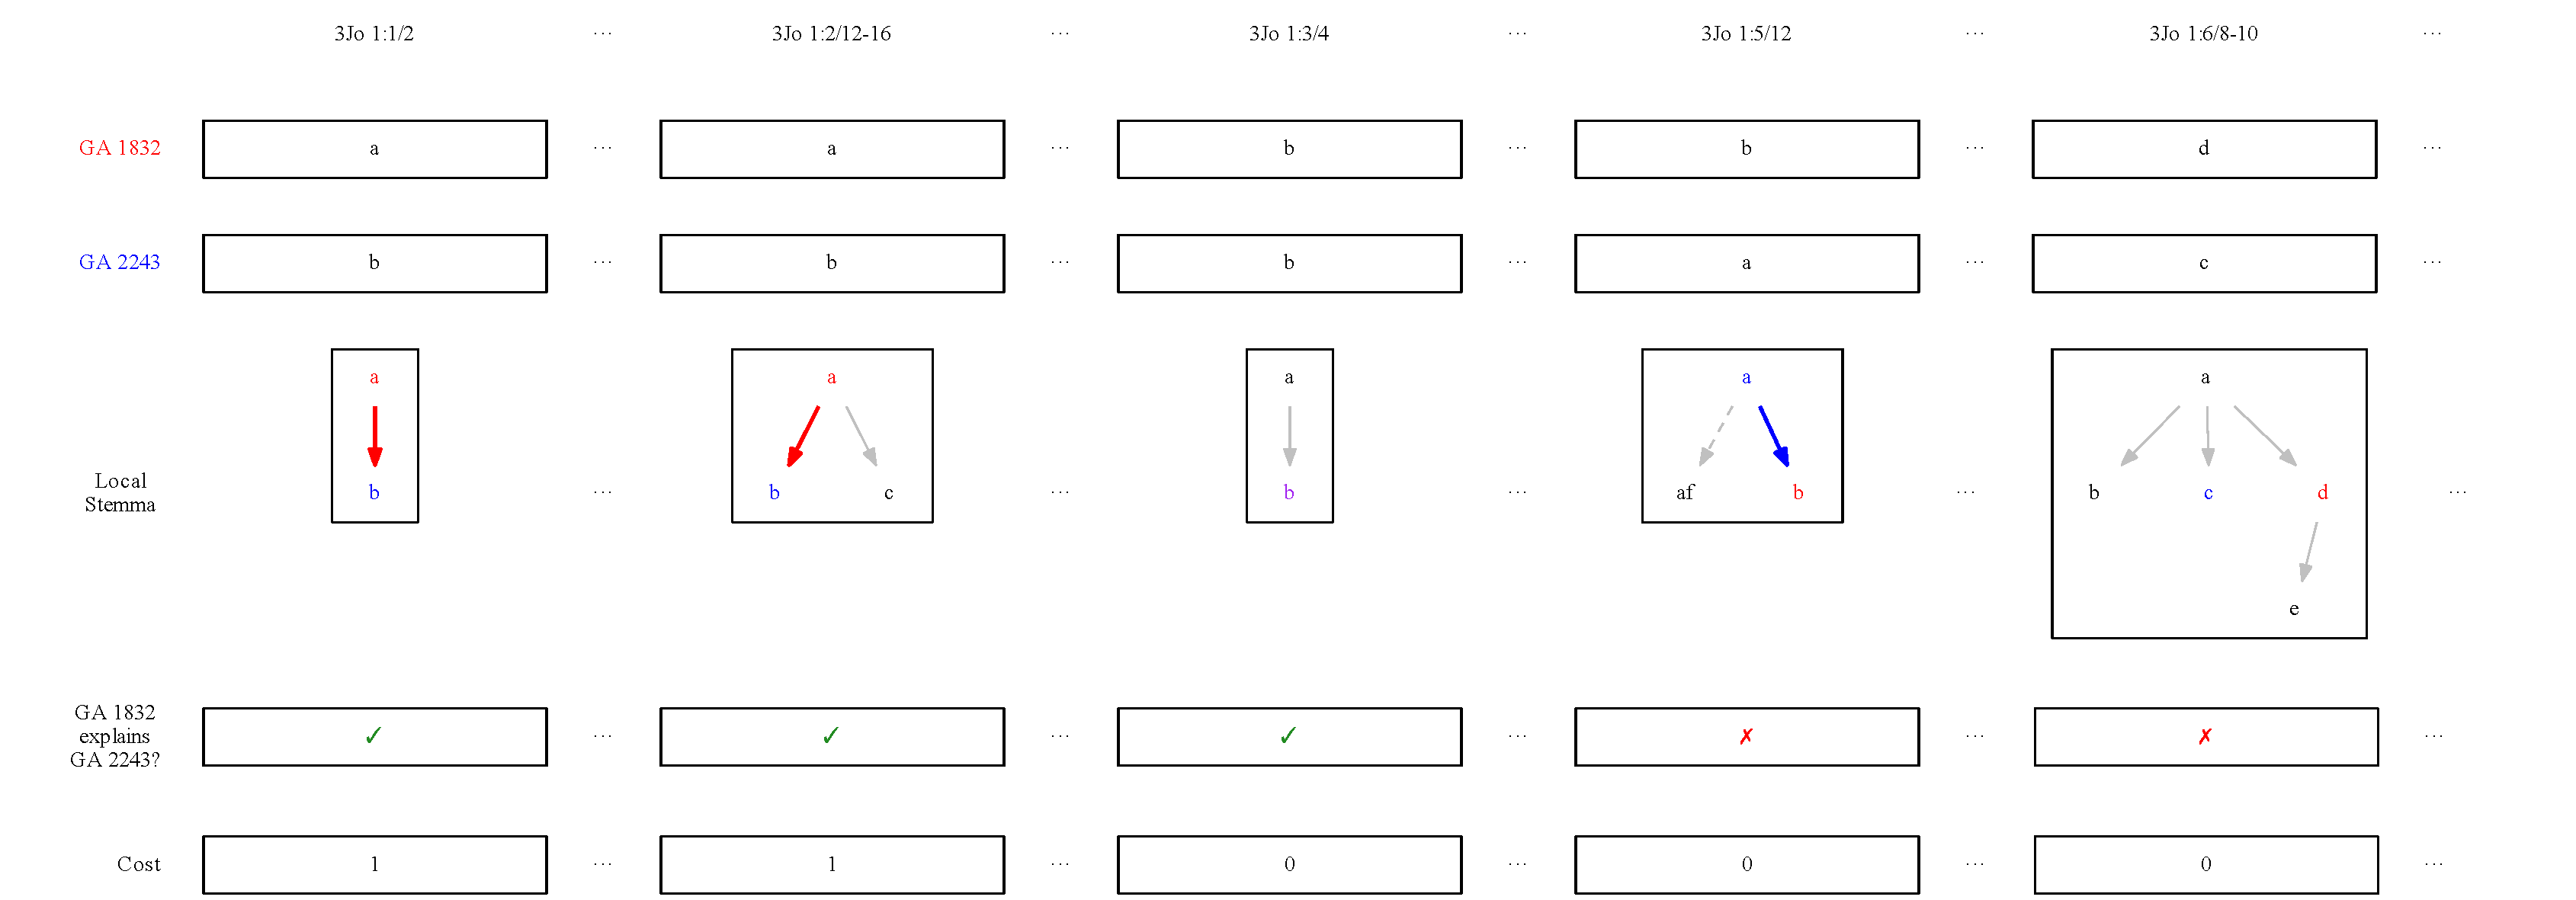
\includegraphics[width=\textwidth]{../img/explained-readings-costs.pdf}
%		\end{center}
%	\end{frame}
%	\begin{frame}
%		\begin{columns}
%			\begin{column}{0.45\textwidth}
%				\begin{itemize}
%					\item If we allow a reading to explain any reading posterior to it, then a better cost per variation unit is the length of the path from the prior reading to the posterior one.
%				\end{itemize}
%			\end{column}
%			\begin{column}{0.45\textwidth}
%				\begin{center}
%					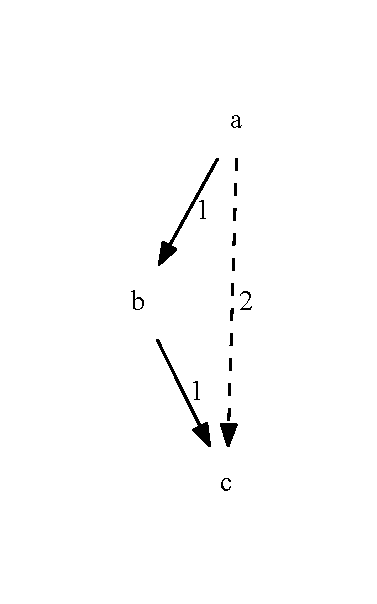
\includegraphics[width=0.75\textwidth]{../img/transitivity-cost.pdf}
%				\end{center}
%			\end{column}
%		\end{columns}
%	\end{frame}
	\section*{Finding a (Good) Substemma}
	\begin{frame}
		\begin{itemize}
			\item Also called \emph{substemma optimization}
			\item For $n$ potential ancestors, a \emph{weighted set cover} problem with $n$ sets (and $2^n - 1$ combinations to check!)
		\end{itemize}
		\begin{center}
			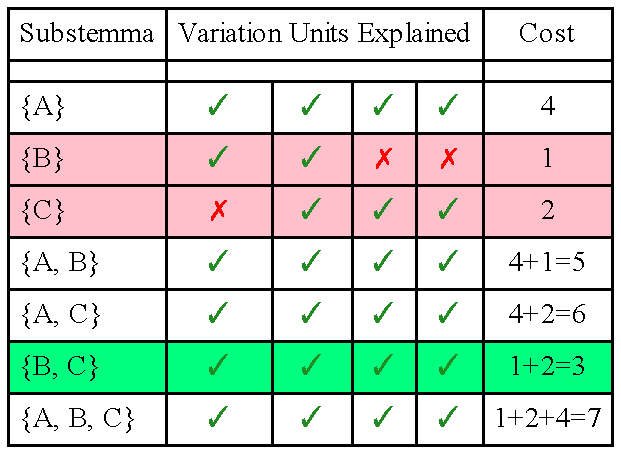
\includegraphics[width=0.75\textwidth]{../img/weighted-set-cover.pdf}
		\end{center}
	\end{frame}
	\begin{frame}
		\begin{columns}
			\begin{column}{0.4\textwidth}
				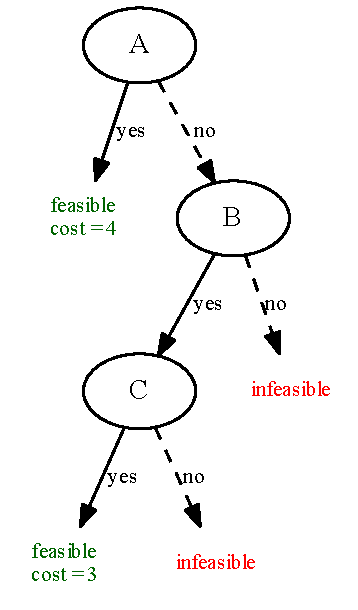
\includegraphics[width=\textwidth]{../img/branch-and-bound-example.pdf}
			\end{column}
			\begin{column}{0.55\textwidth}
				\begin{itemize}
					\item If a witness has many potential ancestors, then checking all $2^n - 1$ possible substemmata by brute force is prohibitive
					\item The \emph{branch-and-bound} heuristic (pictured left) finds all minimum-cost substemmata quickly in practice
					\item Easily adapted to find all substemmata within a given cost
				\end{itemize}
			\end{column}
		\end{columns}
	\end{frame}
	\section*{The Global Stemma}
	\begin{frame}
		\begin{columns}
			\begin{column}{0.45\textwidth}
				\begin{itemize}
					\item Just as the local stemma relates readings, the \emph{global stemma} relates witnesses
					\item Combination of all substemmata into a single graph
				\end{itemize}
			\end{column}
			\begin{column}{0.45\textwidth}
				\begin{center}
					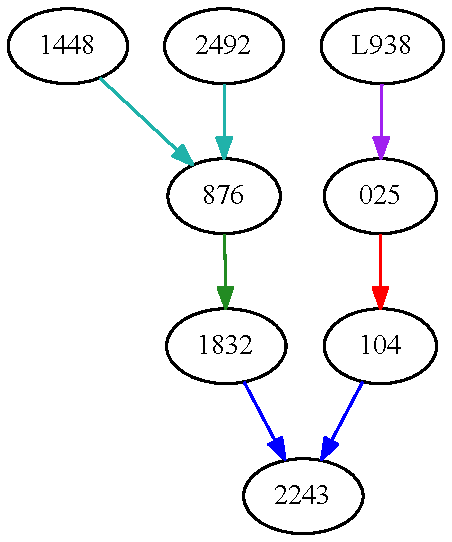
\includegraphics[width=\textwidth]{../img/partial-global-stemma.pdf}
				\end{center}
			\end{column}
		\end{columns}
	\end{frame}
	\begin{frame}
		\begin{columns}
			\begin{column}{0.45\textwidth}
				\begin{itemize}
					\item But \emph{every reading in every local stemma} except the initial one must be explained by another reading
					\item Otherwise…
				\end{itemize}
			\end{column}
			\begin{column}{0.45\textwidth}
				\begin{center}
					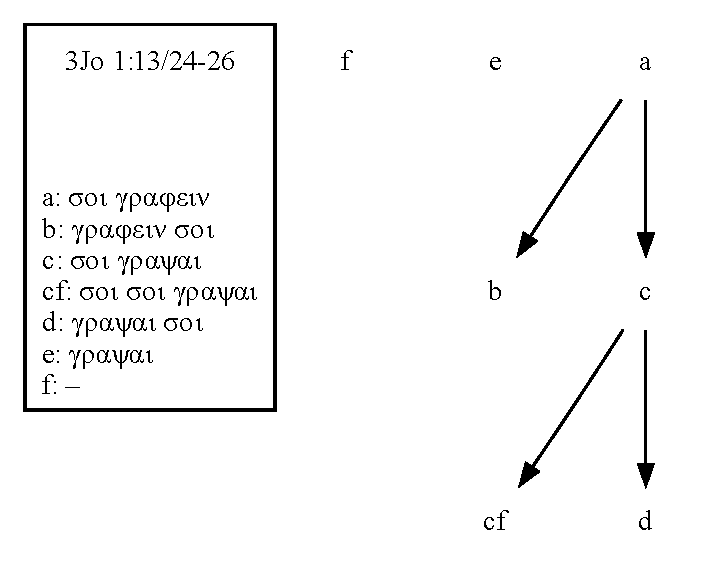
\includegraphics[width=0.875\textwidth]{../img/B25K1V13U24-26-local-stemma-incomplete.pdf}
				\end{center}	
			\end{column}
		\end{columns}
		\begin{center}
			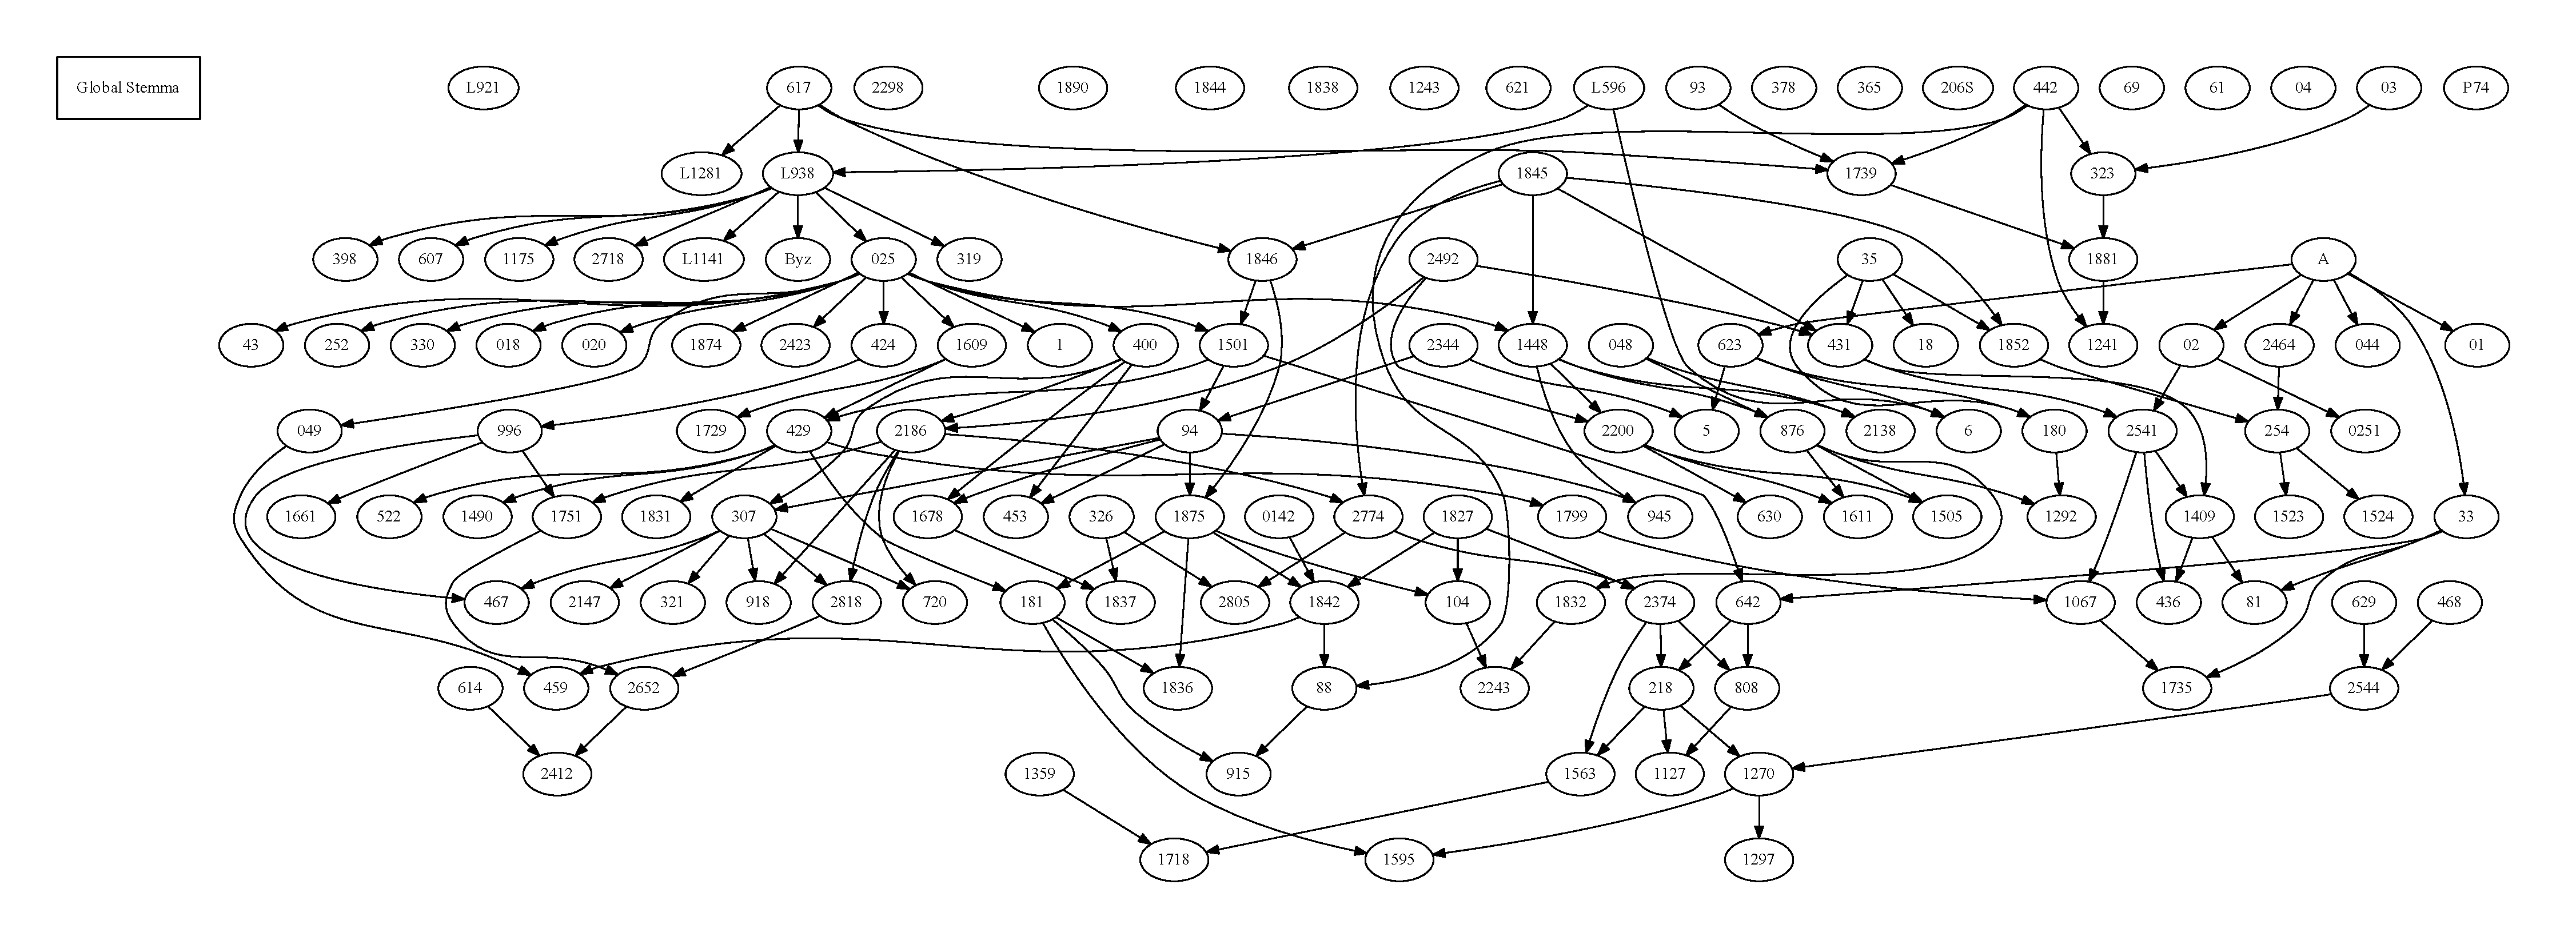
\includegraphics[width=\textwidth]{../img/global-stemma-incomplete.pdf}
		\end{center}	
	\end{frame}
	\begin{frame}
		\begin{columns}
			\begin{column}{0.45\textwidth}
				\begin{itemize}
					\item If we ``complete'' every local stemma (and ignore or manually account for super fragmentary witnesses) ...
				\end{itemize}
			\end{column}
			\begin{column}{0.45\textwidth}
				\begin{center}
					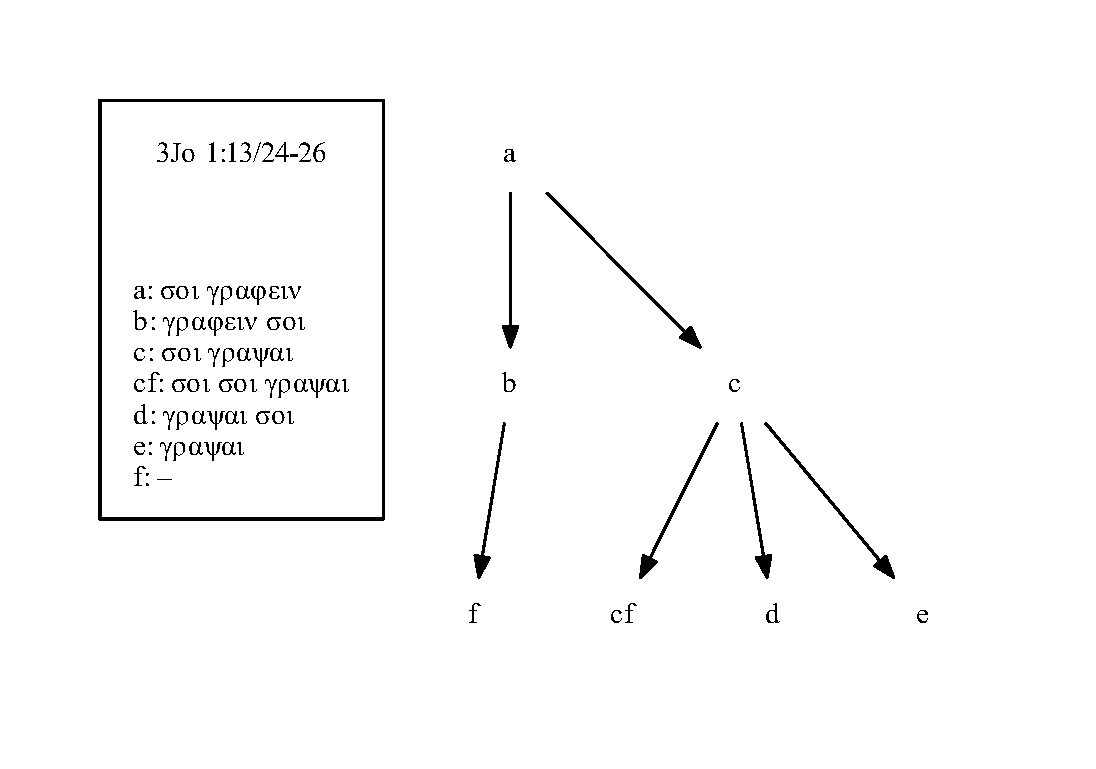
\includegraphics[width=\textwidth]{../img/B25K1V13U24-26-local-stemma-complete.pdf}
				\end{center}	
			\end{column}
		\end{columns}
		\begin{center}
			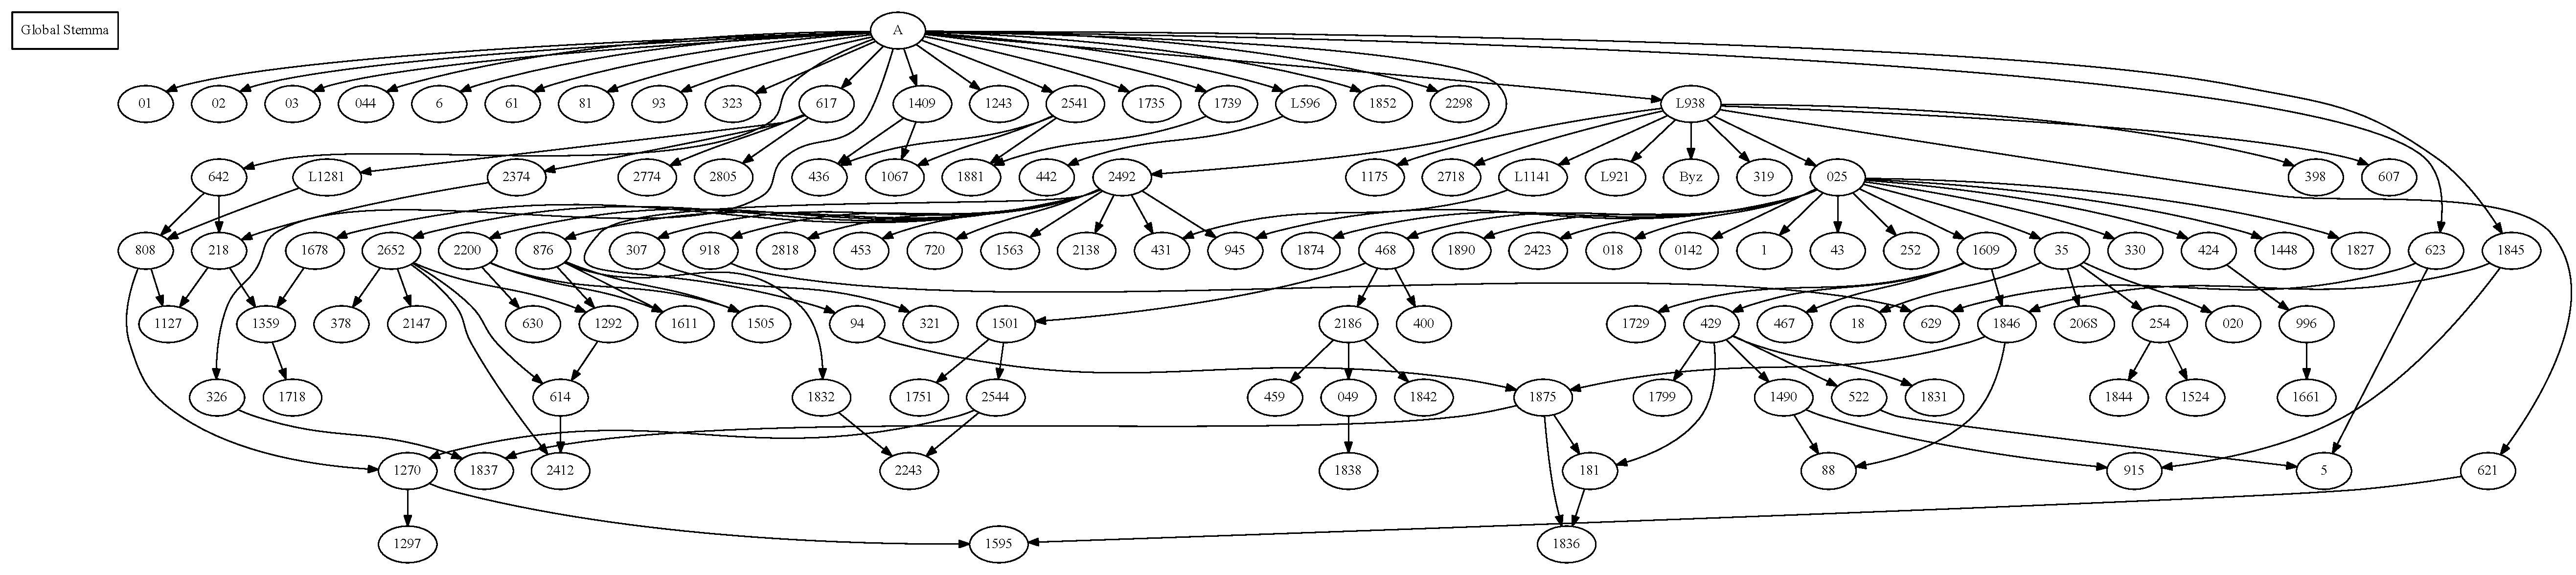
\includegraphics[width=\textwidth]{../img/global-stemma-complete.pdf}
		\end{center}	
	\end{frame}
	\begin{frame}
		\begin{itemize}
			\item How is this different than a textual flow diagram?
			\begin{itemize}
				\item A witness can have more than one ancestor
				\item All readings in a witness must be explained by readings in its ancestor(s)
				\item More computationally intensive, so takes a bit longer to produce
			\end{itemize}
		\end{itemize}
		\begin{center}
			\href{../img/global-stemma-complete-reoriented.pdf}{*Field trip*}
		\end{center}
	\end{frame}
%	\section*{Criticisms and Idiosyncrasies}
%	\begin{frame}
%		\begin{itemize}
%			\item Biggest idiosyncrasy: \emph{no reconstruction of hypothetical ancestors} (because contamination is assumed to make this impossible)
%			\begin{itemize}
%				\item (Personal opinion: this assumption is made for practical rather than theoretical reasons)
%				\item Texts of extant witnesses = bad representatives of ancestors of other extant texts
%				\item CBGM may see ``contamination'' where there's just a gap in the textual tradition
%				\item Enough of the tradition is lost to make this a problem
%			\end{itemize}
%			\item Can the global stemma be understood as a history of the text?
%		\end{itemize}
%	\end{frame}
%	\begin{frame}
%		\begin{itemize}
%			\item Recommended reading:
%			\begin{itemize}
%				\item \cite{Jongkind14}
%				\item The special feature articles in \emph{TC} 20 (2015)
%				\item \cite{Gurry18}
%				\item \cite{Carlson20} (but see \href{http://ntvmr.uni-muenster.de/en_US/intfblog/-/blogs/remarks-on-carlson-a-bias-at-the-heart-of-the-cbgm-guest-post-by-gerd-mink-}{Mink's response})
%			\end{itemize}
%		\end{itemize}
%	\end{frame}
	\section*{Making It Digital}
	\begin{frame}
		\begin{itemize}
			\item The \texttt{open-cbgm} library (my implementation of the CBGM, based on these principles) is freely available at \url{https://github.com/jjmccollum/open-cbgm}, and the standalone command-line utility is available at \url{https://github.com/jjmccollum/open-cbgm-standalone}
			\begin{itemize}
				\item Supported on Windows, Mac, and Linux
			\end{itemize}
			\item The INTF's official implementation (using a Docker container) is now also available (download and instructions at \url{http://ntvmr.uni-muenster.de/intfblog/-/blogs/download-the-cbgm-docker-container})
		\end{itemize}
	\end{frame}
	\section*{Bibliography}
	\begin{frame}[allowframebreaks]
		\printbibliography
	\end{frame}
\end{document}